\documentclass[11pt]{article}
\usepackage[letterpaper,margin=1in]{geometry}
\usepackage[T1]{fontenc}
\usepackage{lmodern}
\usepackage{amsmath,amssymb,amsthm,mathtools}
\usepackage{microtype}
\usepackage{enumitem}
\usepackage{xcolor}
\usepackage{tikz}
\usetikzlibrary{arrows.meta,positioning,calc,fit,decorations.pathreplacing}
\PassOptionsToPackage{hyphens}{url}
\usepackage[unicode,colorlinks=true,linkcolor=blue!45!black,
 citecolor=blue!45!black,urlcolor=blue!45!black]{hyperref}
\hypersetup{pdftitle={Quantum Depletion for Fixed Bounded Repulsive Potentials},pdfauthor={OpenAI}}
\newtheorem{theorem}{Theorem}[section]
\newtheorem{proposition}[theorem]{Proposition}
\newtheorem{lemma}[theorem]{Lemma}
\newtheorem{corollary}[theorem]{Corollary}
\theoremstyle{definition}
\newtheorem{definition}[theorem]{Definition}
\theoremstyle{remark}
\newtheorem{remark}[theorem]{Remark}
\numberwithin{equation}{section}
\newcommand{\R}{\mathbb R}
\newcommand{\N}{\mathbb N}
\newcommand{\Z}{\mathbb Z}
\newcommand{\E}{\mathbb E}
\newcommand{\Pp}{\mathbb P}
\newcommand{\1}{\mathbf 1}
\newcommand{\dd}{\,\mathrm d}
\DeclareMathOperator{\Tr}{Tr}
\DeclareMathOperator{\supp}{supp}
\DeclareMathOperator{\dist}{dist}
\newcommand{\cL}{\mathcal L}
\newcommand{\cC}{\mathcal C}
\newcommand{\cD}{\mathcal D}
\newcommand{\dGamma}{\mathrm d\Gamma}
\newcommand{\manuscriptid}[1]{\nolinkurl{#1}}
\Urlmuskip=0mu plus 1mu\relax
\setlist{itemsep=.25em,topsep=.4em}
\emergencystretch=1em
\clubpenalty=10000
\widowpenalty=10000
\displaywidowpenalty=10000
\title{Quantum Depletion for Fixed Bounded Repulsive Potentials}
\author{OpenAI}
\date{October 5, 2026}
\begin{document}
\maketitle
\begin{abstract}
We prove the Bogoliubov quantum-depletion asymptotic for the ground state
of a three-dimensional Bose gas with a fixed bounded, nonnegative, radial
interaction of finite range and positive scattering length $a$.
The thermodynamic limit is taken at each fixed density $\rho$ before the
dilute limit. Every thermodynamic accumulation value of the fraction
outside the constant mode is
$\frac{8}{3\sqrt\pi}\sqrt{\rho a^3}+o(\sqrt{\rho a^3})$ as
$\rho\downarrow0$. The assertion is uniform over ground-state density
matrices and does not require the occupation to have a unique
thermodynamic limit.
\end{abstract}
\section{Introduction}\label{sec:introduction}

Repulsive interactions move particles out of a Bose condensate even at
zero temperature. For a dilute three-dimensional gas, Bogoliubov theory
predicts a universal leading depletion, depending on the interaction
only through its scattering length. We establish this prediction for
fixed bounded radial repulsive potentials of finite range. The volume
tends to infinity at each fixed density before the density tends to zero.

\subsection{The model and the result}

We use units in which $\hbar^2/(2m)=1$. Let
$v:\R^3\to[0,\infty)$ be bounded, measurable, radial, and compactly
supported, and suppose that $v$ is nonzero on a set of positive measure.
Its scattering length $a_v>0$ is determined by the radial solution of
\[
 (-\Delta+\tfrac12v)f=0,
 \qquad f(x)=1-\frac{a_v}{|x|}
 \quad\text{for sufficiently large }|x|.
\]
On the torus $\Lambda_L=(\R/L\Z)^3$, set
\[
 v_L(x)=\sum_{z\in\Z^3}v(x+Lz),
 \qquad
 H^v_{N,L}=\sum_{j=1}^N(-\Delta_j)
                   +\sum_{i<j}v_L(x_i-x_j),
\]
acting on $L^2_{\mathrm{sym}}(\Lambda_L^N)$ with periodic boundary
conditions. Write $\mathcal G^v_{N,L}$ for the positive trace-one
operators supported on its lowest eigenspace. For
$\Gamma\in\mathcal G^v_{N,L}$, define
\[
 \gamma^{(1)}_\Gamma=N\Tr_{2,\ldots,N}\Gamma,
 \qquad u_0=L^{-3/2},
 \qquad
 B_\Gamma=\frac{\langle u_0,\gamma^{(1)}_\Gamma u_0\rangle}{N}.
\]
Thus $B_\Gamma$ is the occupation fraction of the constant orbital and
$1-B_\Gamma$ is its depletion.

\begin{theorem}\label{thm:main}
For every potential $v$ satisfying the assumptions above and every
$\epsilon>0$, there is $\rho_0(v,\epsilon)>0$ such that, for every fixed
$0<\rho<\rho_0(v,\epsilon)$ and every sequence
$N_k,L_k\to\infty$ with $N_k/L_k^3\to\rho$,
\[
 \limsup_{k\to\infty}\ \sup_{\Gamma\in\mathcal G^v_{N_k,L_k}}
 \left|\frac{1-B_\Gamma}{\sqrt{\rho a_v^3}}
                       -\frac8{3\sqrt\pi}\right|\le\epsilon.
\]
\end{theorem}

The potential remains fixed throughout both limits. In particular, the
statement applies to every thermodynamic accumulation value of the
occupation; existence of an occupation limit at each positive density
is not required. Neither monotonicity of the radial potential nor
positivity of its Fourier transform is assumed. Boundedness makes the
finite-volume heat semigroup positivity improving, so the ground state
is in fact unique. The formulation with density matrices records the
occupation observable without a choice of ground-state vector.

\subsection{Historical context and antecedents}

Bogoliubov's quasiparticle theory describes the excitations and depletion
of a weakly interacting condensate~\cite{Bogoliubov}. Lee, Huang, and
Yang calculated the leading depletion and the second-order energy of
a dilute hard-sphere gas~\cite{LHY}. The two predictions concern
different features of the many-particle ground state: its energy and
its one-body density matrix. In the ordinary thermodynamic limit,
long-wavelength particles can have arbitrarily small kinetic energy.
Consequently, an accurate energy expansion does not by itself determine
the occupation of the constant orbital.

The rigorous energy theory began with Dyson's upper and lower bounds
for hard spheres~\cite{Dyson}. Lieb and Yngvason proved the matching
leading lower bound for repulsive interactions~\cite{LiebYngvason}.
Yau and Yin obtained the Lee--Huang--Yang upper bound for smooth
repulsive potentials~\cite{YauYin}; Basti, Cenatiempo, and Schlein
extended the upper bound to nonnegative radial compactly supported
$L^3$ interactions, with a power-saving remainder~\cite{BCSUpper}.
Fournais and Solovej proved the corresponding lower bound, first for
integrable interactions and then in a class including hard
cores~\cite{FS2020,FS2023}. The sharp hard-sphere upper bound was
subsequently obtained by Basti, Brooks, Cenatiempo, Olgiati, and
Schlein~\cite{BBCOS}. For the present class of potentials, we use the
upper bound of~\cite[Theorem~1.1]{BCSUpper} and retain the additional
positive operators in a local lower bound to recover occupation
observables.

Condensation and depletion are also understood in regimes where the
spatial and dilute limits are linked. Lieb and Seiringer proved complete
condensation for trapped gases in the Gross--Pitaevskii
limit~\cite{LS2002}. Boccato, Brennecke, Cenatiempo, and Schlein
determined the depletion in a periodic unit box with scattering length
of order $N^{-1}$~\cite[Appendix~A]{BBCS}. Their answer is a discrete
Bogoliubov momentum sum. Results of Fournais and later developments
extend condensation estimates to boxes larger than the healing
length~\cite{Fournais2021,Junge2026}. Such estimates do not directly
control the ordinary thermodynamic limit, in which the one-particle
gap closes at every fixed density. For fixed bounded interactions,
the companion~\cite{C} establishes condensation at sufficiently small
fixed densities and sufficiently low positive temperatures, and supplies
the local density tails used here.
The companion~\cite{D} establishes the depletion asymptotic for hard
spheres. The present proof adapts its separation of local energy
estimates from long-distance comparisons to bounded interactions.

Several established methods enter that adaptation. The energy analysis
uses scattering-renormalized positive squares, Neumann localization,
and Bogoliubov diagonalization, as developed in~\cite{FS2020,FS2023}
and in the low-temperature free-energy work
\cite{HHNST,FJGMOTr}. The coherent-state substitution has the standard
upper-symbol corrections of Lieb, Seiringer, and
Yngvason~\cite{LSY2005}. The probabilistic comparison averages a change
of law over routes before taking its moments. This has a direct
antecedent in the deletion-tolerance argument of Peres and
Sly~\cite[Proposition~2.1]{PeresSly}. Its geometric ingredient is the
unpredictable-path method of Benjamini, Pemantle, and
Peres~\cite{BPP}, which produces paths with exponentially decaying
intersection tails. The precise finite-volume version, with rare
encounters away from an endpoint, is supplied by
\cite[Proposition~7.1]{D}.

\subsection{From local occupations to the constant mode}

Here is the obstruction and the division of the proof. Let $\Psi$ be
the positive normalized ground function. For a partition of the torus
into cubes of side $\ell$, let $P_\ell$ be the one-particle projection
onto functions constant on each cube, and let $P_0$ project onto the
single global constant. Since $P_0\le P_\ell$, the depletion splits
exactly as
\begin{equation}\label{eq:intro-split}
 1-B_{|\Psi\rangle\langle\Psi|}
 =\langle\Psi,(1-P_\ell)_1\Psi\rangle
                    +\|(P_\ell-P_0)_1\Psi\|^2.
\end{equation}
The subscript indicates action on the first particle. The first term
measures variations inside the cubes; the second measures variations
between their mean values.

For a suitable mesoscopic choice of $\ell$, Section~\ref{sec:energy}
determines the first term at the depletion scale, together with second
and fourth moments of particle counts.
The argument follows the occupation estimates in
\cite[Section~3]{D}, but deals directly with the bounded potential.
In particular, the Neumann mirror interaction is compared with the
original interaction in expectation using a two-particle bound. This
avoids a pointwise radial-monotonicity comparison. The local lower
bound retains both a kinetic gap and positive quasiparticle terms;
these are needed to transfer the energy calculation to the one-body
observable in~\eqref{eq:intro-split}.

The second term requires information that is uniform in the total
volume. To obtain it, condition a distinguished particle to lie in a specified
cube and integrate out its position. The resulting law of the other
$N-1$ particles has density proportional to the cube average of $\Psi^2$.
Comparing these deletion laws controls the spatial variation of the
root mean squares of $\Psi$. A local comparison of deletion laws,
together with a fine-scale energy estimate, then connects those root
mean squares to the arithmetic means appearing in $P_\ell\Psi$.

Sections~\ref{sec:paths}--\ref{sec:long-palm} perform these comparisons
using ground-state Brownian paths. The construction pairs the
midpoints of paths in two copies so that deleting different endpoint
particles leaves exactly the same observed particles. For a bounded
interaction the conditional path law has Boltzmann weights. We
represent each weight by an auxiliary uniform-variable test and keep
these tests in every conditional normalization. This gives the exact
interacting law while allowing the collision estimates used in the
hard-sphere construction. The density tails of
\cite[Lemmas~4.2 and~4.3]{C} replace the deterministic count
bounds available for hard spheres.

Two different accuracies are needed. A fourth-moment comparison between
neighboring small cubes controls the passage from fine to coarse
averages. A second-moment comparison between distant cubes controls
the remaining variation across the entire torus. For the latter,
routes may have arbitrarily many steps. The estimate therefore charges
only encounters between two independently sampled routes, rather than
one fixed loss at each step. In the copy used to measure the change of law, paths near the common
endpoint remain unchanged. The route theorem makes encounters between
the changed portions rare. These conditional-law and normalization
estimates extend the local and distant comparisons of
\cite[Sections~5,~6, and~8]{D} to bounded repulsion; the hard-sphere
depletion theorem itself is not an input.

Section~\ref{sec:setup} fixes the scales and states the density-tail
inputs. Section~\ref{sec:energy} proves the local occupation and count
estimates, Section~\ref{sec:paths} constructs the conditional path law,
and Sections~\ref{sec:local-palm} and~\ref{sec:long-palm} prove the two
deletion comparisons. Section~\ref{sec:assembly} combines them through
\eqref{eq:intro-split} and restores the original units and order of
limits.

\section{Scales, density tails, and ground-state paths}\label{sec:setup}

We first choose units in which the interaction range is small, the particle
density is large, and the healing length is of order one. Two local
density-tail estimates will then supply the moment and pair bounds used
throughout the paper. Their first use is to control the boundary correction
in the energy calculation of Section~\ref{sec:energy}.

\subsection{Ground states and scaled variables}

For finite $N,L$, the potential in the Hamiltonian is a bounded
multiplication operator. The heat kernel on the labelled configuration
torus is strictly positive, and the Feynman--Kac formula preserves this
positivity. Compact resolvent and positivity improvement therefore give a
unique normalized positive ground function. Permutations of coordinates
and simultaneous translations commute with the Hamiltonian. Uniqueness
implies that this ground function is symmetric and translation invariant.
In particular the bosonic ground space is one-dimensional. We shall use
positivity when comparing spatial arithmetic means with root mean squares
in Section~\ref{sec:assembly}.

Let $R_v>0$ contain the support of the physical potential $v$, and use a
length unit $\sigma>0$. In the resulting coordinates set
\begin{equation}\label{eq:scaled-variables}
 \begin{gathered}
 K=L/\sigma,\qquad V=K^3,\qquad D=N/V,\qquad a=a_v/\sigma,\\
 \alpha=Da,\qquad r=R_v/\sigma,\qquad W(y)=\sigma^2v(\sigma y).
 \end{gathered}
\end{equation}
The scaled Hamiltonian has kinetic energy $-\Delta$ and pair potential
$W$, periodized on the torus of side $K$. Its normalized positive ground
function is denoted by $\Phi$, and
\[
 \mu(\dd X)=\Phi(X)^2\dd X.
\]
Integrals in all particle coordinates use Lebesgue measure. We write
$\langle O\rangle_\psi=\langle\psi,O\psi\rangle$; this notation does not
normalize a vector that is not already normalized.

Fix a sufficiently large constant $B_0$, depending on $v$, and put
\begin{equation}\label{eq:physical-base-scale}
 \sigma_*=B_0\rho^{-1/2},\qquad
 D_*=\rho\sigma_*^3=B_0^3\rho^{-1/2},\qquad
 \alpha_0=a_vB_0^2.
\end{equation}
Along the thermodynamic sequence we choose $\sigma\to\sigma_*$, as
specified below. Then $D\to D_*$ and $\alpha\to\alpha_0$. All estimates
are uniform for $\alpha$ in a fixed compact positive neighborhood of
$\alpha_0$. Constants may depend on the fixed potential and this
neighborhood. In these units,
\begin{equation}\label{eq:potential-scales}
 a\asymp r\asymp D^{-1},\qquad
 \int_{\R^3}W\le C D^{-1},\qquad 0\le W\le C D^2.
\end{equation}
A bounded measurable radial potential can be replaced by a Borel version
with its range and radial bounds holding everywhere. Such null changes
affect neither the operator nor the Brownian path integrals.

Choose small exponents $u>0$ and $0<w<u/10000$, and let
\begin{equation}\label{eq:partition-scales}
 R=\lceil D_*^w\rceil,\qquad
 B=R\lceil D_*^u/R\rceil,\qquad d=1/j\quad(j\in\N).
\end{equation}
The fixed microcell size $d$ resolves variation within cells.  The
slowly growing scale $R$ is used for the distant deletion comparison,
while the still larger $B$-boxes give the energy calculation room to
resolve variation on the $R$-scale.  For each fixed $j$, the dilute
hierarchy is $r\ll d\le1\ll R\ll B$.  All partition sizes are fixed
during the thermodynamic limit, when $K\to\infty$; $j$ is sent to
infinity only after the estimates at each fixed $j$.

The restrictions on $u$ arise in the energy estimates; it may be taken
smaller than $10^{-9}$ and decreased further there. The path exponent
$x>0$ will be chosen after $u,w$. At fixed $\rho$, choose $K$ to be the
nearest positive multiple of $B$ to $L/\sigma_*$ and set $\sigma=L/K$.
This gives the asserted convergence of $\sigma$ on a tail of every
thermodynamic sequence.

We use nested cubic partitions $\cC_l$ of the scaled torus for
$l=B,R,1,d$. Unit cells $U_z$ are centered at
$z\in\cL=(\Z/K\Z)^3$, with compatible half-open conventions on
boundaries. If $A$ is a spatial set, $n_A$ denotes its particle count.
Let $P_l$ be the one-body orthogonal projection onto functions constant
on every cell of $\cC_l$, and set
\begin{equation}\label{eq:cell-projections}
 W_l=1-P_l,\qquad \dGamma(O)=\sum_{i=1}^N O_i.
\end{equation}
Thus $W_l$ is a projection, whereas $W$ without a subscript is the pair
potential. Averages over cells or cell pairs are uniform unless a
different measure is specified.

\paragraph{Limit convention.}
We always take the thermodynamic limsup at fixed $\rho$ first, followed
by $\rho\downarrow0$, equivalently $D_*\to\infty$. A term $o_K(1)$
tends to zero in the first limit; a dilute $o(1)$ tends to zero after
that limsup. Power bounds in $D$ hold for all sufficiently large $D_*$
and sufficiently far in the corresponding inner sequence. Terms tending
to zero only in the inner limit can therefore be absorbed into a stated
power bound on a tail. No uniform rate in that sequence is required.
Constants and thresholds in estimates involving $d$ may depend on the
fixed integer $j$.

\subsection{Local density tails}

We use two results from the bounded-interaction companion~\cite{C}.
We record both the physical form of the input and the consequence needed
here, so that the dependence on temperature and volume is explicit.
For a canonical Gibbs state let its position law be the diagonal of its
density matrix.

\begin{proposition}[Density-tail input from \cite{C}]\label{prop:density-input}
Let $v$ satisfy the hypotheses of Theorem~\ref{thm:main}. There is a
sufficiently large fixed $B_0$ such that, for all sufficiently small
$\rho>0$, the following statements hold at physical base length
$b=B_0\rho^{-1/2}$ and count scale $n=\rho b^3$.
\begin{enumerate}[label=\textup{(\roman*)}]
\item If the particle density is at most $2\rho$, let
$A=\sum_i g(x_i)$, where $0\le g\le1$, the support of $g$ is covered
by $J$ base cubes, and $|\nabla g|^2\le C_gb^{-2}g$ almost everywhere
for a prescribed fixed bound on $C_g$. Then
\[
 \Pp(A>M)\le C e^{-cM},\qquad M\ge CnJ.
\]
Sharp counts have such majorants after a fixed enlargement and a fixed
increase in $J$.
\item If the density lies in $[\rho/2,2\rho]$ and $Q_1,\ldots,Q_J$
are cubes of side $b$ with centers separated by a sufficiently large
fixed multiple of $b$, then
\[
 \Pp\left(\sum_{i=1}^J n_{Q_i}\le\epsilon_0 nJ\right)
 \le e^{-c_1 nJ}
\]
for fixed $\epsilon_0,c_1>0$.
\end{enumerate}
Both assertions hold in all sufficiently large volumes, uniformly down
to arbitrarily small positive temperatures. Their volume thresholds do
not grow as temperature decreases. Fixed positive multiplicative changes
in cube sides are allowed after changing constants, and $B_0$ can be
increased to meet any finite list of lower bounds.
\end{proposition}

The density-tail inputs are supplied by the localized density and occupation
estimates of~\cite[Lemmas~4.2 and~4.3]{C}; for the upper tail we take
exponential parameter one.
Their proofs use local energy and entropy estimates and a localized
replacement argument. They do not require a condensation or depletion
conclusion. Their temperature uniformity lets us apply them to the
ground state at each fixed finite volume: canonical Gibbs states converge
in trace norm to its rank-one projection as temperature tends to zero.

\begin{lemma}[Scaled count tails]\label{lem:count-tails}
After fixing $B_0$ and decreasing $\rho$ if necessary, there are positive
constants $c,c',C$ such that, for every nonempty $A\subset\cL$,
\begin{equation}\label{eq:count-tails}
 \begin{aligned}
 \Pp_\mu\left(\sum_{z\in A}n_{U_z}\ge b\right)
   &\le C e^{-cb},&& b\ge CD|A|,\\
 \Pp_\mu\left(n_{U_z}<c'D\text{ for every }z\in A\right)
   &\le e^{-cD|A|}.
 \end{aligned}
\end{equation}
\end{lemma}
\begin{proof}
The physical side of a scaled unit cell is $\sigma\to b$, and
$D\asymp D_*$. A fixed enlargement covers any union of the given unit
cells by $O(|A|)$ base cubes, proving the first bound from
Proposition~\ref{prop:density-input}(i). For the second, a bounded coloring
of the unit lattice extracts a subset of $A$ of size at least $c_0|A|$
whose cells have the separation required in part (ii). If every original
count is below $c'D$, their sum on this subset is below the threshold of
part (ii) when $c'$ is small enough. The allowed fixed side adjustments
handle either sign of $\sigma-b$. The actual physical density eventually
lies in $[\rho/2,2\rho]$. This proves both claims uniformly on a tail
of the thermodynamic sequence.
\end{proof}

For $A\subset\cL$ define
\[
 F_A(X)=\sum_{i=1}^N e^{-d_K(x_i,A)},\qquad F_\varnothing=0,
\]
where $d_K$ denotes torus distance and the sites of $A$ are regarded as
points of the torus. The tails imply the exponential moment bound
\begin{equation}\label{eq:count-mgf}
 \log\E_\mu e^{hF_A}\le ChD|A|\qquad(0\le h\le h_*),
\end{equation}
for a fixed $h_*>0$. Indeed the upper tail first gives this statement
for the sharp count in a site set and one small positive value of $h$;
convexity extends it to the interval from zero. The sites at distance at
most $m+1$ from $A$ number at most $C(1+m)^3|A|$. Write the exponentially
weighted count as a sum of counts in these enlargements, with exponentially
decaying coefficients. Jensen's inequality with normalized summable weights
and the sharp-count bound prove~\eqref{eq:count-mgf}. The same proof works
if distance is multiplied by any fixed positive constant.

In particular, each fixed $q$th moment of a count in a fixed number of
unit cells is $O(D^q)$. Counts in polynomially many cells have polynomial
fixed moments. If one of those cells exceeds a sufficiently large fixed
multiple of $D$, its probability is exponentially small in $D$.
Cauchy--Schwarz therefore makes every fixed product of these counts on
that exceptional event smaller than every power of $D^{-1}$. We will use
this observation when removing count cutoffs.

\subsection{Ground-state paths and local pair bounds}

Let $E_m$ be the ground energy of $m$ particles on the scaled torus,
with the same potential $W$. Adjoining a constant last coordinate to a
normalized $(m-1)$-particle trial function gives
\begin{equation}\label{eq:removal-energy}
 E_m-E_{m-1}\le\frac{m-1}{V}\int W\le C
 \quad(m\le N),\qquad E_N-E_{N-m}\le Cm.
\end{equation}
This trial need not be symmetric: the positive ground energy on the
labelled space equals the bosonic ground energy by the uniqueness already
proved.

For $0<T\le1$, consider independent torus Brownian motions on $[-T,T]$
with generator $\Delta$ and initial Lebesgue measure. Weight their joint
law by
\begin{equation}\label{eq:ground-path-law}
 e^{2TE_N}\Phi(\omega(-T))\Phi(\omega(T))
 \prod_{i<k}\exp\left[-\int_{-T}^T
              W(\omega_i(q)-\omega_k(q))\dd q\right].
\end{equation}
Here and below the pair potential in torus expressions is periodized.
The Feynman--Kac formula makes~\eqref{eq:ground-path-law} a probability
measure with marginal $\mu$ at every time. Restrictions to shorter slabs
are consistent, by the ground-state eigenfunction identity.

\begin{lemma}[Free-path domination]\label{lem:path-domination}
If $m$ specified labels carry nonnegative single-path weights $H_i$ that
are invariant under time reversal, then under~\eqref{eq:ground-path-law},
\begin{equation}\label{eq:path-domination}
 \E\prod_{i=1}^m H_i(\omega_i)
 \le e^{Cm}\int\mu(\dd Y)
                  \prod_{i=1}^m\E^{Y_i}_{\mathrm{free}}H_i.
\end{equation}
A weight without reversal symmetry can be replaced by the sum of itself
and its reversal.
\end{lemma}
\begin{proof}
Delete every interaction incident to the specified labels; nonnegativity
of $W$ increases the integral. Fix their initial and final coordinates
$y,z$. The remaining semigroup has norm $e^{-2TE_{N-m}}$, so the integral
in the other labels is bounded by that norm times $g(y)g(z)$, where
$g(y)$ is the $L^2$ norm of the slice $\Phi(y,\cdot)$. The product of
the free weighted endpoint kernels is symmetric in $y,z$ by reversal
invariance. Thus $g(y)g(z)\le(g(y)^2+g(z)^2)/2$ replaces the slice
product by its initial square after integration. Since $g(y)^2$ is the
specified-coordinate marginal of $\mu$, the result follows from
\eqref{eq:removal-energy}. Truncation proves the assertion for unbounded
nonnegative weights.
\end{proof}

Apply this lemma on the longer slab $[-1,1]$. At any time $|q|\le1/2$,
the probability for a free path started at $Y_i$ to lie in a cube of
side $h\le1$ within a fixed distance of a site $z$ is bounded by
$Ch^3e^{-2d_K(Y_i,z)}$, by the torus heat kernel. The bound also holds
for the reversed observation. Summing~\eqref{eq:path-domination} over
distinct labels and using~\eqref{eq:count-mgf} shows that two specified
such cubes have expected ordered pair count at most $CD^2h^6$.
Covering a fixed site neighborhood by $h$-cubes and summing over the
bounded number of neighboring cubes for each one gives
\begin{equation}\label{eq:pair-bound}
 \E\#\{(i,k):i\ne k,\ X_i,X_k\text{ in the neighborhood},\
                    d_K(X_i,X_k)\le h\}\le CD^2h^3.
\end{equation}
These bounds are uniform in the site and in the observation time on the
central slab. They provide the required short-distance control using only
the imported count tails and the elementary removal-energy estimate.

\section{Energy and mesoscopic occupation}\label{sec:energy}

The energy comparison has two outputs: concentration of local particle
counts and the occupation outside functions constant on mesoscopic cells.
The latter determines the depletion except for wavelengths larger than
$R$.  The path comparisons in the following sections will control that
remaining contribution.  Throughout this section $\langle\cdot\rangle_\psi$
denotes the quadratic form in $\psi$, without division by $\|\psi\|^2$.
For a spatial cell $A$, put $q_A=n_A/(D|A|)$.

\begin{proposition}[Local energy outputs]\label{prop:local-energy}
Choose $u>0$ sufficiently small and then $0<w<u/10000$, with the
partitions of Section~\ref{sec:setup}.  In the stipulated order of
thermodynamic and dilute limits, the ground vector satisfies
\begin{equation}\label{eq:local-energy}
\begin{aligned}
 \E_{A\in\cC_R}\langle(q_A-1)^2\rangle_\Phi
       &\le CD^{-1-w/6},&
 \E_{A\in\cC_d}\langle(q_A-1)^4\rangle_\Phi
       &\le C_jD^{-1-u/6},\\
 V^{-1}\langle\dGamma(W_R)\rangle_\Phi
       &=\frac8{3\sqrt\pi}\alpha^{3/2}+o(1),&
 V^{-1}\langle\dGamma(W_d)\rangle_\Phi
       &\le\epsilon_j+o_j(1),\qquad \epsilon_j\longrightarrow0.
\end{aligned}
\end{equation}
The parameter $j$ is fixed before taking these limits.  Constants are
uniform for $\alpha$ in the fixed compact positive window.
\end{proposition}

The organization of the comparison follows the mesoscopic energy
argument of \cite[Section~3]{D}.  Its scattering-square decomposition and
Neumann cosine analysis are related to
\cite[Sections~2 and~5]{FJGMOTr}.  We give the needed estimates for the
present interaction, including the wall correction and cubic cancellation.
In particular the proof uses the bounded potential $W$ itself.

\subsection{The upper bound and Neumann boxes}

Put $c_{\rm L}=128/(15\sqrt\pi)$ and define, holding $a$ fixed when taking
derivatives,
\[
 e(y)=4\pi ay^2+4\pi c_{\rm L}a^{5/2}y^{5/2}.
\]
The Lee--Huang--Yang upper bound of
\cite[Theorem~1.1]{BCSUpper} applies because the fixed physical potential
is radial, nonnegative, compactly supported and belongs to $L^3$.
Its error is $O(\rho^{5/2+c})$ for some $c>0$, with a constant depending
on that potential.  Under our rescaling energy density is multiplied by
$\sigma^5$, and $\rho\asymp D^{-2}$.  Consequently, for some $c_*>0$,
\begin{equation}\label{eq:energy-upper}
 E_N\le V\bigl(e(D)+O(D^{-c_*})\bigr).
\end{equation}
As elsewhere, this denotes a bound on the thermodynamic limsup; no
finite-volume convergence rate is required.  To pass from the Dirichlet
upper bound to any periodic density-convergent sequence, place a
Dirichlet trial box inside the periodic box with a range margin and
side ratio tending to one.  Use a slightly larger fixed density there,
so its particle number eventually exceeds the desired one.  Slicing out
excess coordinates and averaging cannot increase the energy, since the
omitted kinetic and interaction forms are nonnegative.  Extending the
remaining slices by zero respects the periodic form domain and the range
margin makes the interactions agree.  Let the larger density decrease
to the prescribed density, using continuity of the explicit upper bound.
This proves \eqref{eq:energy-upper} along the sequences used here.

We use the same box estimates at two scales: $E=R$ yields the coarse
count variance, and $E=B$ yields the microcell fourth moment and both
occupation estimates.  For a generic box side $E$, abbreviate $Q=E$
and $v_b=E^3$.
Thus $Q\asymp D^\theta$ for $\theta=u$ or $w$.  Restrict configuration
space to sectors assigning each label to a box and discard interactions
between boxes.  These are Neumann form restrictions: we restrict gradient
integrals, without differentiating the sector indicators.  Each local
vector is symmetric in the labels assigned to its box, and may take
values in the Hilbert space of the spectator coordinates.

It is convenient to reflect the interaction at each wall.  For a radial
function $g$ supported in $\{|x|\le r\}$ define on $[0,E]^3$
\[
 g^s(x,y)=\sum_{z\in\Z^3}g(p_z(x)-y),
\]
where, coordinatewise, $p_z$ maps $[0,E]^3$ onto the cube translated by
$Ez$, reversing a coordinate precisely when the corresponding $z_i$ is
odd.  Write $H_b$ for the Neumann Hamiltonian with pair potential $W^s$.
The added mirror terms are nonnegative, but their expectation on the
original ground vector is small:
\begin{equation}\label{eq:energy-mirror-error}
 \sum_b\langle H_b\rangle\le E_N+CV/E.
\end{equation}
Indeed an added interaction requires two particles within $Cr$ of each
other and within $Cr$ of a wall.  Its multiplicity is bounded.  At most
$C(V/E)r^{-2}$ cubes of side comparable with $r$ cover all walls.  The
small-cube pair estimate proved before \eqref{eq:pair-bound} gives
$CD^2r^6$ ordered pairs per such cube, and $\|W\|_\infty\le CD^2$.
Since $r\asymp D^{-1}$, the resulting bound is $CV/E$.
All later excitation localizations use this same mirror Hamiltonian.

Let $u_p$, $p\in(\pi/E)\N_0^3$, be the real normalized Neumann cosines:
\[
 u_p(x)=v_b^{-1/2}\prod_{i=1}^3c_{p_i}\cos(p_ix_i),\qquad
 c_0=1,\quad c_s=\sqrt2\ (s>0).
\]
Even extension shows that the integral operator with kernel $g^s$ has
eigenvalue $\widehat g(p)$ on $u_p$, with Fourier convention
$\widehat g(p)=\int g(x)e^{-ip\cdot x}\,\dd x$.  In particular its row
integral is the constant $\widehat g(0)$.
Write $a_p,a_p^*$ for the corresponding bosonic operators and set
\begin{equation}\label{eq:energy-bands}
 J=Q^{100},\qquad
 n_+=\sum_{p\ne0}a_p^*a_p,\qquad
 n_L=\sum_{0<|p|\le J/E}a_p^*a_p,\qquad
 n_H=n_+-n_L,\qquad M\asymp Dv_bQ^{-400}.
\end{equation}
Take $M$ integral.  We refer to $0<|p|\le J/E$ as the low band and the
remaining nonzero modes as the high band.  All power inequalities below
hold if $u$ is sufficiently small, for example $u<10^{-9}$ and
sufficiently small relative to $c_*$.  Further decreases are harmless.

\subsection{A rough bound retaining count and kinetic penalties}

We first obtain a lower bound with an error much larger than the
Lee--Huang--Yang term.  Its purpose is to control vectors with many
excitations, leaving only a small-excitation sector for the sharper
calculation.  The construction is the radial replacement and small-box
method of Dyson and Lieb--Yngvason~\cite{Dyson,LiebYngvason}, with an
explicit reserve of kinetic energy.

\begin{lemma}[Rough box bound]\label{lem:energy-rough}
For $0\le n\le6Dv_b$, as a quadratic-form inequality on the bosonic
$n$-particle Neumann space,
\begin{equation}\label{eq:rough-energy}
\begin{split}
 H_b\ge{}&\frac{4\pi an^2}{v_b}-Cv_bD^{1-0.001}
       +c\,\dGamma(\min\{p^2,1\})\\
 &+cD\sum_{A\in\cC_d,\ A\subset b}|A|
    \mathfrak h\left(q_A-\frac{n}{Dv_b}\right),
 \qquad \mathfrak h(y)=\frac{y^2}{1+|y|}.
\end{split}
\end{equation}
The same inequality holds with Hilbert-space-valued spectator variables.
\end{lemma}

\begin{proof}
We can discard the mirror terms for this estimate.  Subdivide each
$d$-cell into equal cubes of side $\ell\asymp D^{-0.31}$, and put
$b_1=D^{-0.36}$ and $\xi=D^{-0.002}$.  For large $D$, $r<b_1/2$.
Restrict to the corresponding assignment sectors and drop interactions
between small cubes.

Split the kinetic coefficient as $1=(1-2\xi)+\xi+\xi$.
The radial replacement below uses the first term only within distance
$b_1$ of another particle in the small cube.  We use one $\xi$ reserve
for Temple's inequality and retain the other for the kinetic term in
\eqref{eq:rough-energy}; outside those neighborhoods the first term
also remains available.

Fix one particle coordinate and all the others in its small cube.
Partition the cube into the Voronoi regions of those other particles,
clipped at the walls.  Each region is star-shaped about its center.
The radial scattering variational principle on a ray gives, for
$R'\ge r$,
\begin{equation}\label{eq:energy-ray}
 \int_0^{R'}\bigl((1-2\xi)|f'(s)|^2+\tfrac12W(s)|f(s)|^2\bigr)
                  s^2\,\dd s
 \ge(1-2\xi)a|f(R')|^2.
\end{equation}
With kinetic coefficient one the exact endpoint minimum is
$a(1-a/R')^{-1}|f(R')|^2$: integrate the scattering equation against its
regular solution, then complete the quadratic form around the minimizer.
To obtain \eqref{eq:energy-ray}, first bound the potential term below by
$(1-2\xi)W/2$, and then discard $(1-a/R')^{-1}\ge1$.
No monotonicity of the radial function $W$ is involved.

Let $U$ be constant on $b_1/2<|x|<b_1$, zero elsewhere, and normalized
by $\int U=4\pi$.  Average \eqref{eq:energy-ray} over radii available
on each ray with weight $U(R')(R')^2\,\dd R'$.  The weight has total at
most one.  Integrating the rays replaces the short-distance energy by
$(1-2\xi)aU(d_{\rm nn})$, where $d_{\rm nn}$ is the nearest-neighbor
distance in the small cube; the expression is zero when there is no
neighbor.  Assigning half of each pair potential to each endpoint uses
no interaction twice.  This argument first holds for smooth vectors
and then by form approximation.

In a small cube with $k\le C_0D\ell^3$ particles, the mean of the
replacement sum in its normalized constant vector is at least
\[
 \frac{4\pi(1-2\xi)ak(k-1)}{\ell^3}
       \left(1-C\frac{b_1}{\ell}-C\frac{kb_1^3}{\ell^3}\right).
\]
For this estimate put one coordinate at least $b_1$ from the walls,
integrate a possible nearest neighbor over the shell, and exclude closer
neighbors by the union bound.  Distinct choices of the nearest neighbor
are disjoint outside null sets.  The replacement sum is nonnegative
and bounded by $Ckab_1^{-3}\le CD^{0.15}$.  Its variance in the constant
vector is therefore at most this upper bound times its mean.  The
kinetic gap supplied to Temple's inequality is
$\pi^2\xi/\ell^2\asymp D^{0.618}$.
Temple's inequality yields the lower bound
\[
 \frac{4\pi a}{\ell^3}(1-CD^{-0.002})k(k-1).
\]
Here the other relative errors are
$b_1/\ell=O(D^{-0.05})$ and $Db_1^3=D^{-0.08}$; the variance correction
is smaller still.  The formula also holds for $k=0,1$.

For $k>C_0D\ell^3$, partition the labels into groups of sizes between
$C_0D\ell^3/3$ and $C_0D\ell^3$, allowing integer rounding, and drop
intergroup interactions.  Choose a fixed cutoff $b_*>12$, and then $C_0$
sufficiently large.  With
\[
 F(y)=\begin{cases}y^2,&0\le y\le b_*,\\2b_*y-b_*^2,&y>b_*,\end{cases}
\]
the same estimate in every number sector is bounded below by
\[
 \frac{4\pi a}{\ell^3}(1-CD^{-0.002})
       \left[(D\ell^3)^2F\left(\frac{k}{D\ell^3}\right)-k\right].
\]
Indeed $F(y)\le y^2$ below the group threshold, whereas above it the
group estimate has a linear coefficient larger than $2b_*D\ell^3$.
For $\vartheta=n/(Dv_b)\in[0,6]$,
\[
 F(y)\ge\vartheta^2+2\vartheta(y-\vartheta)
                         +c\mathfrak h(y-\vartheta),\qquad y\ge0.
\]
Below $b_*$ the remainder is a square.  Above $b_*$, writing
$s=y-\vartheta$ and $a_0=b_*-\vartheta>0$, it is
$2a_0s-a_0^2\ge a_0s$.  This proves the displayed comparison uniformly.
Summing small cubes cancels the tangent deviations.  The self-count
terms cost at most $Ca\ell^{-3}n\le Cv_bD^{0.93}$, and the relative
loss in the leading scalar costs $Cv_bD^{1-0.002}$.
Convexity of $\mathfrak h$ and Jensen's inequality inside each $d$-cell
now give the scalar and count terms of \eqref{eq:rough-energy}.

It remains to recover a fixed amount of the indicated kinetic form.
The preceding construction leaves coefficient $\xi$ everywhere and
$1-2\xi$ outside the $b_1$-neighborhoods of the other particles.
For a coordinate slice enlarge those neighborhoods to their union $S$;
then $|S|\le Cnb_1^3$.  The vector fields $\nabla u_p/|p|$ are orthonormal.
Their projection $\Pi$ for $0<|p|\le D^{0.003}$ has squared evaluation
norm at most $CD^{0.009}$.  Hence, by duality,
\[
 \|\Pi\1_S F\|_2^2\le CD^{0.009}nb_1^3\|F\|_2^2
                \le CD^{-0.071}Q^3\|F\|_2^2=o(\xi)\|F\|_2^2.
\]
Apply this to $F=\nabla f$ and use
$\|\Pi F\|_2^2\le2\|\1_{S^c}F\|_2^2+2\|\Pi\1_SF\|_2^2$.
Neumann integration by parts identifies the projected gradient norm
with $\sum_{0<|p|\le D^{0.003}}p^2|\langle u_p,f\rangle|^2$.
Above this cutoff the everywhere reserve suffices because
$\xi p^2\ge D^{0.004}$.  Sum over coordinates.  This last argument is
on the original Neumann form domain of the $E$-box, after summing back
the small-cube restrictions; it does not impose artificial Neumann
conditions on an arbitrary collection of small-cube functions.
\end{proof}

\subsection{Restricting the excitation number}

The cutoff below is a finite-band instance of the matrix localization
method of \cite[Appendix~A]{LiebSolovej}.  We give its form estimate
directly so that the retained positive terms remain explicit.

Comparing Lemma~\ref{lem:energy-rough} with the tangent to
$4\pi ay^2$ at $D$, and using \eqref{eq:energy-upper} and
\eqref{eq:energy-mirror-error}, gives the preliminary estimate
\begin{equation}\label{eq:energy-preliminary}
 V^{-1}\sum_{b,\ n\le6Dv_b}\langle n_+\rangle\le CQ^2D^{1-0.001}.
\end{equation}
For completeness the higher number sectors do not spoil this comparison:
partition their labels into groups of sizes between $2.5Dv_b$ and
$6Dv_b$, apply the rough bound to each group and drop intergroup
interactions.  The energy per particle is then at least
$10\pi\alpha-o(1)$, exceeding the tangent slope $8\pi\alpha$ by a
fixed positive amount.  Thus those sectors have a surplus of order $n$.
For $n\le6Dv_b$, the scalar tangent remainder is nonnegative and
$\min(p^2,1)\ge cE^{-2}$ on the nonconstant modes, proving
\eqref{eq:energy-preliminary}.

Localize only the middle number sectors
\[
                       Dv_b/2\le n\le6Dv_b.
\]
Choose real Lipschitz functions $f,h$ with $f^2+h^2=1$, $f=1$ below
$M/8$, $f=0$ above $M/4$, and Lipschitz constants at most $C/M$.
The three localizing operators are
\begin{equation}\label{eq:energy-cutoffs}
 F_1=f(n_L)^2,\qquad F_2=h(n_L)^2,\qquad F_3=\sqrt2f(n_L)h(n_L).
\end{equation}
They have $\sum F_i^2=1$.  The first and third pieces are supported on
$n_L\le M/4$ and will be called low pieces; the second is supported on
$n_L\ge M/8$.  Also $\psi=F_1\psi+F_2\psi$, which later transfers
count estimates even though counts need not commute with these cutoffs.
Finite-rank smooth one-body projections preserve the Neumann form domain.

Here is the localization error, with $V_n^s$ the sum of mirror pair
potentials:
\begin{equation}\label{eq:energy-cutoff-error}
 \left|\sum_{i=1}^3\langle H_b\rangle_{F_i\psi}
                      -\langle H_b\rangle_\psi\right|
 \le\frac C{M^2}\left(\langle V_n^s\rangle_\psi
       +\|W\|_1\frac{J^3}{v_b}n\langle n_+\rangle_\psi\right).
\end{equation}
To prove it, let $\Pi_k$ project onto $n_L=k$.  Kinetic energy commutes
with the cutoffs, and the potential has block width two.  The difference
of its forms is
\[
 -\frac12\sum_{k,l,i}(F_i(k)-F_i(l))^2
                       \langle\Pi_k\psi,V_n^s\Pi_l\psi\rangle.
\]
Positivity, form Cauchy--Schwarz and the finite block width bound this
by $CM^{-2}$ times the block-diagonal expectation.  The latter is the
phase average of $e^{-isn_L}V_n^se^{isn_L}$.  For a pair only the two
coordinate rotations matter.  Expanding each as
$1+(e^{is}-1)P_L$, every additional term has a low projection on at
least one coordinate.  The evaluation bound
$P_L(x,x)\le CJ^3/v_b$ and the constant row integral of $W^s$ give
\[
 P_{L,i}W^s(x_i,x_k)P_{L,i}
       \le C\|W\|_1J^3v_b^{-1}P_{L,i}.
\]
Expanding squared norms and summing pairs proves
\eqref{eq:energy-cutoff-error}.
The analogous error for $\dGamma(A)$, $\|A\|\le1$, is at most
$CnM^{-2}\|\psi\|^2$, by block width one and its norm bound $n$.

The summed potential expectation is $O(VD)$, including the mirror
correction.  Together with \eqref{eq:energy-preliminary},
\eqref{eq:energy-cutoff-error} has total error $O(VQ^{-1})$.
Even replacing $\|W\|_1\le C/D$ by the weaker $CQ$ gives the per-volume
bound
\[
 O\bigl(D^{-1}Q^{794}+D^{-0.001}Q^{1097}\bigr)=O(Q^{-1}).
\]
All these inequalities include sector weights and spectator integration.

\subsection{The sharp box estimate}

We now analyze a low piece.  The aim is to recover the
Lee--Huang--Yang scalar while retaining two positive terms: a weak
particle-excitation gap and a quasiparticle energy.  The latter will
identify the occupation observable.

Let $\varphi$ be the scattering function of $W$, and set
\[
 \omega=1-\varphi,\qquad g=W\varphi,\qquad m=g\omega.
\]
The maximum principle and the radial scattering equation give
$0\le\varphi\le1$, $\widehat g(0)=8\pi a$ and $\|m\|_1\le C/D$.
For $p\ne0$ put
\begin{equation}\label{eq:energy-tau}
 S=E^{-2}(n_++Jn_H),\qquad
 \tau_p=p^2-E^{-2}\bigl(1+J\1_{\{p\ \text{high}\}}\bigr).
\end{equation}
Thus $\tau_p\asymp p^2$.  For the constant mode use coherent vectors
$|z\rangle=e^{-|z|^2/2}\sum_{q\ge0}z^q|q\rangle/\sqrt{q!}$,
measure $\dd\lambda(z)=\pi^{-1}\dd^2z$, and coherent projections
$\psi_z=\langle z|\psi\rangle$ onto the excitation Fock space.
For $|z|^2\le2n$ define
\[
 \rho_z=|z|^2/v_b,\qquad t_p=\rho_z\widehat g(p),\qquad
 D_p=(\tau_p^2+2t_p\tau_p)^{1/2}.
\]
These roots are positive: $|t_p|\le C$, while $\widehat g(p)\ge0$ on
every fixed momentum ball for large $D$, by positivity and shrinking
support.  Large $p$ are controlled by $\tau_p\asymp p^2$.
After rotating excitation modes by the phase of $z$, the change of
variables used below diagonalizes the one-mode quadratic form
\[
 (\tau_p+t_p)a_p^*a_p+\tfrac12t_p(a_p^2+a_p^{*2}).
\]
Specifically, define $b_p$ through
\begin{equation}\label{eq:energy-bogoliubov}
\begin{gathered}
 a_p=U_pb_p+V_pb_p^*,\qquad U_p>0,\quad U_p^2=1+V_p^2,\\
 V_p^2=\tfrac12\left(\frac{\tau_p+t_p}{D_p}-1\right),\qquad
 2U_pV_p=-t_p/D_p.
\end{gathered}
\end{equation}
With this choice,
\[
 (\tau_p+t_p)a_p^*a_p+\tfrac12t_p(a_p^2+a_p^{*2})
  =D_pb_p^*b_p+\tfrac12(D_p-\tau_p-t_p).
\]
The formulas with $z=0$ have $U_p=1,V_p=0$.

\begin{lemma}[Sharp energy with positive remainders]\label{lem:energy-sharp}
If $Dv_b/2\le n\le6Dv_b$ and $\psi$ is supported on $n_L\le M/4$,
then
\begin{equation}\label{eq:sharp-energy}
\begin{split}
 \langle H_b\rangle_\psi\ge{}&
 \bigl(v_be(n/v_b)-Cv_bQ^{-1/4}\bigr)\|\psi\|^2+c\langle S\rangle_\psi\\
 &+c\int_{|z|^2\le2n}\sum_{p\ne0}\widetilde D_p
                       \|b_p\psi_z\|^2\,\dd\lambda(z),\\
 &\hspace{12mm}\widetilde D_p=D_p\ \text{on the low band},\qquad
 \widetilde D_p=D_p/J\ \text{on the high band}.
\end{split}
\end{equation}
\end{lemma}

The proof has three parts.  Scattering-square splitting produces a
quadratic Hamiltonian and a cubic term.  Its quadratic vacuum energy is
the Lee--Huang--Yang scalar.  Completing the high-frequency cubic square
creates a contraction that cancels against the retained $m$ term.
We supply each part, since the cancellation must leave the positive
remainders in \eqref{eq:sharp-energy}.

\begin{proof}[Proof of Lemma~\ref{lem:energy-sharp}]
\emph{Scattering-square splitting.}
Let $P=|u_0\rangle\langle u_0|$, $Z=P_i^\perp P_j^\perp$ and $A=1-Z$.
For every summand in the mirror kernel, with its argument suppressed,
there is the exact identity of forms
\begin{equation}\label{eq:energy-scattering-square}
 W=(Z+\omega A)^*W(Z+\omega A)+ZgA+AgZ+A(g+m)A.
\end{equation}
It follows by expanding, using $g=W(1-\omega)$ and
$m=W\omega(1-\omega)$.
In the cubic blocks $P_iP_j^\perp g^sZ$ and their adjoints retain only
the low projection in coordinate $j$.  The high remainder costs a small
fixed fraction of the positive squares and $Cn_H$.  Here is a direct
verification.  In each mirror term substitute
$Z=(Z+\omega A)-\omega A$.  Cauchy--Schwarz against the square bounds
the first part by that square plus $Cn_H$: the latter bound uses
$g^2/W\le W$, the constant row integral of $W^s$, and
$n\|W\|_1/v_b\le C$.  The other part contains $m^sA$.
Between $P_iP_j^{\rm high}$ and
$A=P_iP_j+P_iP_j^\perp+P_i^\perp P_j$ its first block vanishes.
Its other blocks act only on high modes, by the constant row integral
for the direct block and cosine diagonalization for the exchange block.
Their norms are at most $\|m\|_1/v_b$, again giving $Cn_H$ after summing.
This is absorbed by $E^{-2}Jn_H$ since $J/E^2\to\infty$.

The retained $g$ direct terms in the number-$n$ sector combine into
\begin{equation}\label{eq:energy-number-term}
 \frac{\widehat g(0)}{2v_b}
            \{n(n-1)-n_+(n_+-1)\}.
\end{equation}
After separating $S$, the remaining terms are
\begin{equation}\label{eq:energy-retained-hamiltonian}
\begin{split}
 &\frac{\widehat m(0)}{2v_b}a_0^{*2}a_0^2\\
 &+\sum_{p\ne0}\left[
  \tau_pa_p^*a_p+
  \frac{\widehat g(p)+\widehat m(p)+\widehat m(0)}{v_b}
                           a_0^*a_p^*a_pa_0
  +\frac{\widehat g(p)}{2v_b}(a_0^{*2}a_p^2+a_p^{*2}a_0^2)\right]\\
 &+\frac1{v_b}\sum_{\substack{p\ \text{low}\\ k,l\ne0}}
 C_{pkl}\widehat g(k)
                (a_0^*a_p^*a_la_k+a_k^*a_l^*a_pa_0),
 \qquad C_{pkl}=\sqrt{v_b}\int_bu_pu_ku_l.
\end{split}
\end{equation}
These are the matrix elements of
\eqref{eq:energy-scattering-square}: the constant mode paired through
$g^s$ with mode $k$ leaves exactly the triple cosine coefficient in the
last line.  Blocks with just one nonconstant index vanish.  The
coefficients $C_{pkl}$ are bounded, and fixing any two indices leaves at
most a fixed number of possible third indices.  These facts follow
coordinatewise from the product-to-sum identity for cosines.  We keep
these exact coefficients, including modes with zero components.

On the present excitation cutoff,
\begin{equation}\label{eq:energy-number-square}
 n_+^2\le C(Mn_++nn_H).
\end{equation}
Thus replacing \eqref{eq:energy-number-term} by $4\pi an^2/v_b$ costs
$O(1)\|\psi\|^2$ and an $o(1)$ fraction of $S$.
For example its two excitation coefficients are $O(Q^{-400})$ on
$n_+$ and $O(1)$ on $n_H$, compared with $E^{-2}$ and $JE^{-2}$.

\emph{Coherent resolution.}
Use the resolution of the identity in the zero mode.  The upper symbols
of $a_0^*a_0$ and $a_0^{*2}a_0^2$ are respectively
$|z|^2-1$ and $|z|^4-4|z|^2+2$; these follow by scalar gamma integration,
or see \cite{LSY2005}.  Hence in
\eqref{eq:energy-retained-hamiltonian} we may substitute $z,\bar z$
for $a_0,a_0^*$, with total integrated error $O(1)\|\psi\|^2$.
Indeed the Fourier coefficients are $O(D^{-1})$, $n\le6Dv_b$, and
\[
 \int|z|^2\|\psi_z\|^2\,\dd\lambda(z)
       =\langle n-n_++1\rangle_\psi.
\]
The region $|z|^2>2n$ is negligible, also with fixed polynomial weights:
after angular integration its radial variables are gamma variables
with integer shapes at most $n+1$, whose tails there are exponentially
small.  All negative terms, estimated without kinetic energy, have
polynomial operator bounds on sectors with at most $n$ excitations.
For the pairing terms this follows from Parseval for the bounded mirror
kernel; there are only polynomially many low cubic indices.
The coherent projections preserve both $n_L\le M/4$ and $n_+\le n$.
It therefore suffices to estimate a normalized excitation vector $\eta$
in that subspace, at $|z|^2\le2n$.  For this calculation rotate phases
so that $z$ is real.

\emph{The quadratic vacuum energy.}
Diagonalizing the $g$ quadratic terms gives positive
$\sum D_p\|b_p\eta\|^2$, the remaining $m$ terms, and the scalar
\begin{equation}\label{eq:energy-lhy-scalar}
 \frac12\sum_{p\ne0}(D_p-\tau_p-t_p)
       +\frac12v_b\rho_z^2\widehat m(0)
 =4\pi c_{\rm L}a^{5/2}v_b\rho_z^{5/2}+O(v_bQ^{-1/4}).
\end{equation}
We justify the error without any regularity assumption on $W$.
The equation $-\Delta\omega=g/2$ and the Newton kernel give
\[
 \widehat m(0)=\frac12\int_{\R^3}\frac{\widehat g(k)^2}{|k|^2}
                      \,\dd\bar k,\qquad
                   \dd\bar k=(2\pi)^{-3}\dd k.
\]
Writing $H(k)=\widehat g(k)/(8\pi a)$, the radial sine formula,
$\|g\|_\infty\le CD^2$ and $\supp g\subset\{|x|\le C/D\}$ imply
\begin{equation}\label{eq:energy-fourier-decay}
 |H(k)|\le\min\{1,CD/|k|\},\qquad
 |\nabla H(k)|\le C\min\{D^{-1},|k|^{-1}\}.
\end{equation}
The uniform derivative bound uses the first moment of $g$.
For the large-frequency bounds differentiate
$4\pi\int_0^r g(s)s\sin(|k|s)/|k|\,\dd s$ and use the height and range
bounds; no derivative of $g$ is taken.

Neumann lattice summation in the positive octant gives
\begin{equation}\label{eq:energy-riemann-m}
 \frac1{v_b}\sum_{p\ne0}\frac{H(p)^2}{p^2}
   =\int_{\R^3}\frac{H(p)^2}{p^2}\,\dd\bar p
                    +O\left(\frac{1+\log D}{E}\right).
\end{equation}
To see this, compare cubes of mesh $\pi/E$.  The octant weight
$\pi^{-3}$ equals the full-space weight $(2\pi)^{-3}$ for the even
integrand.  The cubes meeting zero cost $O(E^{-1})$.  Away from zero,
the derivative is bounded by
$C(|p|^{-3}+D^{-1}|p|^{-2})$ up to radius $D$ and by
$C(D^2|p|^{-5}+D|p|^{-4})$ above it.  Shell summation, including face
cubes, proves \eqref{eq:energy-riemann-m}; here $\log E=O(\log D)$.
Thus the second term in \eqref{eq:energy-lhy-scalar} may be replaced
by $\sum t_p^2/(4p^2)$ at the stated accuracy.

Replacing $\tau_p$ by $p^2$ in the first term costs $O(v_b/E)$.
At bounded frequencies the derivative of the summand is bounded by
$C(1+|p|^{-1})$ and the shift is $E^{-2}$.  At large frequencies the
derivative is $O(|p|^{-4})$; the additional high-band shift $J/E^2$
is compensated by summing only above $J/E$.
In the combined summand replace $t_p$ by $t_0=8\pi a\rho_z$.
Above radius $Q$ its absolute tail is $O(Q^{-1})$ per volume by Taylor
expansion.  Below $Q$, positivity and support give
$|t_p-t_0|\le Cp^2/D^2$, while differentiation in $t$ costs at most
$C(1+p^{-2})$.  The summed error is $O(Q^5/D^2)$ per volume.
Finally, the constant-$t_0$ Riemann sum differs from its integral by
$O((1+\log E)/E)$ per volume: near zero use the bounds
$C|p|^{-2},C|p|^{-3}$ for the function and its derivative, and at infinity
use the Taylor bounds $C|p|^{-4},C|p|^{-5}$.
All these errors are $O(Q^{-1/4})$.
The integral equals
\[
 \frac{t_0^{5/2}}{4\pi^2}
 \int_0^\infty x^2
   \left(\sqrt{x^4+2x^2}-x^2-1+\frac1{2x^2}\right)\dd x.
\]
The radial integral is $8\sqrt2/15$, by evaluating an elementary
antiderivative and taking its endpoint limits.  Substitution of
$t_0=8\pi a\rho_z$ proves \eqref{eq:energy-lhy-scalar}, including $z=0$.

The scalar is now correct.  We next control the cubic term while
preserving a fraction of the quasiparticle energy.  The $m$ terms still
present in \eqref{eq:energy-retained-hamiltonian} are essential here.

\emph{The cubic terms with low $k$.}
Put $\lambda=(Dv_b)^{-1/2}$ and $N_+=\langle n_+\rangle_\eta$.
After coherent substitution the cubic coefficients are bounded by
$C\lambda|H(k)|$.  Whenever we sum triples below, $p$ is low and
$C_{pkl}\ne0$.
For low $k$, Cauchy--Schwarz applied to
$\|a_l^*a_p\eta\|$ and $\|a_k\eta\|$ gives
\begin{equation}\label{eq:energy-low-cubic}
 C\lambda J^{3/2}(M+CJ^3)^{1/2}N_+=o(E^{-2})N_+.
\end{equation}
Indeed there are $O(J^3)$ low indices, any two indices have bounded
multiplicity for the third, and
$\|a_l^*a_p\eta\|^2=\|a_la_p\eta\|^2+\|a_p\eta\|^2$.
The double-annihilation sum is bounded by
$\langle n_Ln_+\rangle_\eta$.

\emph{The high $k$ creation part.}
For high $k$ use $a_k=U_kb_k+V_kb_k^*$, with
$|U_k|\le C$ and $|V_k|\le C|H(k)|/k^2$.
Commute $b_k^*$ to the left in the $V_k$ part.  Besides the reordered
term this produces the commutator with $a_l$ when $l=k$; the
commutator with $a_p^*$ vanishes because $p$ is low.  Set
\[
 T_H=\sum_{k\ \text{high}}\frac{k^2}{J}\|b_k\eta\|^2.
\]
There are $O(J^3)$ triples for fixed $k$.  Weighted Cauchy--Schwarz
therefore bounds the reordered term by
\[
 C\lambda J^2 T_H^{1/2}
       \left(\sum_{p,k,l}\frac{H(k)^4}{k^6}
                                \|a_p^*a_l\eta\|^2\right)^{1/2}.
\]
The unweighted squared-norm sum is at most
$C(M+J^3)N_+$, again by cosine multiplicities and commutation.
Young's inequality bounds this by an arbitrarily small fixed fraction
of $T_H$ plus
\begin{equation}\label{eq:energy-high-creation-error}
 C\lambda^2J^4(E/J)^6(M+J^3)N_+=o(E^{-2})N_+.
\end{equation}
For the commutator, $C_{pkk}\ne0$ requires some nonzero component of
$p$ to equal twice the corresponding component of $k$.
For fixed $p$, the sum of $H(k)^2/k^2$ over these high $k$ is at most
$CE^2(1+\log D)$: on each such plane use dyadic shells and the decay
in \eqref{eq:energy-fourier-decay} above $D$.
Its total contribution is at most
\[
 C\lambda E^2(1+\log D)J^{3/2}\sqrt{N_+}.
\]
It costs an arbitrarily small fixed fraction of $E^{-2}N_+$ and the
scalar error $CD^{-1}Q^{303}(1+\log D)^2$.

\emph{The high $k$ annihilation part and its contraction.}
Complete a square between the $U_kb_k$ cubic and the fraction $1-3/J$
of the high diagonal energy.  The resulting negative form is bounded by
\begin{equation}\label{eq:energy-cubic-square}
 \frac{\rho_z}{v_b}\sum_{k\ \text{high}}
  \frac{\widehat g(k)^2U_k^2}{(1-3/J)D_k}
       \left\|\sum_{p,l}C_{pkl}a_l^*a_p\eta\right\|^2.
\end{equation}
Normal ordering separates its quartic and contraction parts.
The absolute value of the quartic part is at most
\begin{equation}\label{eq:energy-cubic-quartic}
 C\lambda^2(E/J)^2J^3\langle n_Ln_+\rangle_\eta
                                      =o(E^{-2})N_+.
\end{equation}
For fixed $p,p'$ the sums over $k,l,l'$ in the products
$\|a_{l'}a_p\eta\|\,\|a_la_{p'}\eta\|$ have bounded multiplicity.
Put $A_p=\sum_{l\ne0}\|a_la_p\eta\|^2$.  Cauchy--Schwarz first
bounds each fixed-$p,p'$ sum by $C\sqrt{A_pA_{p'}}$, and then
\[
 \sum_{p,p'\ {\rm low}}\sqrt{A_pA_{p'}}
 \le \#\{p:p\ {\rm low}\}\sum_{p\ {\rm low}}A_p
 \le CJ^3\langle n_Ln_+\rangle_\eta .
\]
The weight is bounded using $|k|>J/E$.  This proves
\eqref{eq:energy-cubic-quartic}.

The contraction matrix for fixed $k$ has entries
\[
 B^{(k)}_{pp'}=\sum_{l\ne0}C_{pkl}C_{p'kl}
\]
on low modes.  It is positive with bounded norm, since it is the
compression of multiplication by $v_bu_k^2$, whose supremum is at
most eight.  The omitted $l=0$ term is zero when $k$ is high and $p$
is low.  If every component $k_i>2J/E$, the product-to-sum formula for
$u_k^2$ makes this compression exactly the identity.
For all high $k$,
\[
 \frac{U_k^2k^2}{(1-3/J)D_k}\le1+C/J.
\]
The exceptional component slabs satisfy
\begin{equation}\label{eq:energy-slab-sum}
 \frac1{v_b}\sum_{\substack{k\ \text{high}\\\min_i k_i\le2J/E}}
                \frac{H(k)^2}{k^2}
       \le C\frac{J(1+\log D)}E.
\end{equation}
There are $O(J)$ lattice planes per slab; each plane has the same
$CE^2(1+\log D)$ bound used for the commutator.  Combining
\eqref{eq:energy-riemann-m} and \eqref{eq:energy-slab-sum}, the
contraction in \eqref{eq:energy-cubic-square} is at most
\begin{equation}\label{eq:energy-cubic-contraction}
 \left(2\rho_z\widehat m(0)
       +C\left[J^{-1}+D^{-1}J(1+\log D)/E\right]\right)
                                      \langle n_L\rangle_\eta.
\end{equation}
The factor two comes from
$\int\widehat g(k)^2/k^2\,\dd\bar k=2\widehat m(0)$.
On the other hand the low-band $m$ diagonal in
\eqref{eq:energy-retained-hamiltonian}, after coherent substitution,
is at least
\[
 2\rho_z\widehat m(0)n_L-CD^{-2}(J/E)^2n_L.
\]
This uses the second-moment estimate from $\supp m\subset\{|x|\le r\}$.
Its high-band part is nonnegative because
$\widehat m(p)+\widehat m(0)\ge0$ for the nonnegative function $m$.
Thus the leading term in \eqref{eq:energy-cubic-contraction} cancels,
and every remaining coefficient is $o(E^{-2})$.

For clarity, the preceding absorptions have ample strict margins.
The low-$k$ coefficient in \eqref{eq:energy-low-cubic} is bounded by
$C(Q^{-50}+D^{-1/2}Q^{298.5})$; the coefficient in
\eqref{eq:energy-high-creation-error} is
$C(Q^{-594}+D^{-1}Q^{103})$; and
\eqref{eq:energy-cubic-quartic} has coefficient $CQ^{-298}$.
The commutator scalar is $o(v_bQ^{-1/4})$ for sufficiently small $u$.
Completing the main square used only $1-3/J$ of the high diagonal;
the creation estimate uses a small fraction of the remaining
$J^{-1}$ energy.  Thus a fixed multiple of $\widetilde D_p$ remains,
as does a fixed fraction of $S$.

\emph{Integration and domains.}
Integrate the estimates on coherent vectors.  The function
$4\pi c_{\rm L}a^{5/2}\rho^{5/2}$ is convex, and its derivative at
$\rho=n/v_b$ is $O(D^{-1})$.  Its tangent there, together with the
coherent second-moment identity, shows that replacing its integrated
value by the value at $n/v_b$ loses at most
$CD^{-1}(\|\psi\|^2+\langle n_+\rangle_\psi)$.
This is absorbed in the scalar error and the retained $S$.
The gamma tail previously discarded is exponentially small.

All calculations can first be made with finitely many excitation modes.
At fixed parameters the bounded interaction is form-continuous under
finite-mode approximation, which preserves the excitation cutoffs.
The pairing coefficients have square-summable Fourier coefficients by
Parseval, and the cubic has finitely many low indices.  The displayed
bounds justify passage in the completed squares; a positive remainder
can first be retained on finitely many modes and then passed to the
limit by lower semicontinuity.  This proves
\eqref{eq:sharp-energy} on the full form domain.
\end{proof}

\subsection{The energy surplus and count moments}

The sharp estimate now applies to the low pieces; the rough estimate
handles their complement and the outlying particle-number sectors.
The bookkeeping is most transparent relative to the affine function
\[
                  t_b(n)=v_be(D)+e'(D)(n-Dv_b).
\]
Its sum over boxes is exactly $Ve(D)$ in every assignment sector.

\begin{lemma}[Positive quantities paid for by the energy surplus]
\label{lem:energy-surplus}
After summing boxes, assignment sectors, and spectator variables, each
of the following quantities is bounded by $CVQ^{-1/5}$:
\begin{enumerate}
\item the original box-count penalty
$\sum_bDv_b\langle\mathfrak h(n/(Dv_b)-1)\rangle$;
\item on high pieces, the sum of
$\langle\dGamma(\min\{p^2,1\})\rangle$ and
$D\sum_{A\subset b}|A|\langle\mathfrak h(q_A-1)\rangle$;
\item on low pieces, the $S$ form and the integrated positive
quasiparticle form in \eqref{eq:sharp-energy};
\item on number sectors outside $[Dv_b/2,6Dv_b]$, the sum of
$(n+Dv_b)$ times their squared norms.
\end{enumerate}
\end{lemma}

\begin{proof}
On a high piece $n_L\ge M/8$, so its rough kinetic term supplies at
least $cM/E^2$.  This pays for the error $Cv_bD^{1-0.001}$ and the
$O(v_b)$ Lee--Huang--Yang tangent correction: the relevant ratio is
$D^{0.001}Q^{-402}\to\infty$.
A fixed fraction of the kinetic term remains.  The scalar quadratic
remainder controls $Dv_b\mathfrak h(n/(Dv_b)-1)$ in the middle range.
It also recenters the microcell penalty at one, since
$\mathfrak h(s+t)\le C(\mathfrak h(s)+\mathfrak h(t))$ and
$\sum_{A\subset b}|A|=v_b$.

On low pieces convexity of $e$ retains the same box penalty in addition
to the two positive forms of Lemma~\ref{lem:energy-sharp}.
Below the middle range the scalar rough bound exceeds $t_b(n)$ by
$cDv_b$, after its error is absorbed.  Above it the grouping argument
used for \eqref{eq:energy-preliminary} gives a surplus $cn$.
These also control the stated box penalty on the outliers.
Box counts commute with the localizations, so their penalties sum back
to the original restrictions.
Finally combine \eqref{eq:energy-upper},
\eqref{eq:energy-mirror-error}, and \eqref{eq:energy-cutoff-error}.
The total scalar errors are
$O(VQ^{-1/4}+VQ^{-1}+VD^{-c_*})$, which are
$O(VQ^{-1/5})$ after making $u$ small relative to $c_*$.
\end{proof}

At $E=R$, the first conclusion immediately gives a clipped second
moment of $q_b-1$ bounded by $CD^{-1}Q^{-1/5}$.  We next prove the
microcell fourth moment at $E=B$.  This is where retaining the
excitation gap, rather than only the scalar energy, is useful.

For a microcell $A\subset b$, put
\[
 X_A=n_A-n|A|/v_b
     =\dGamma\bigl(\1_A-|A|/v_b\bigr).
\]
Its one-body summand has norm at most one and zero constant-mode
diagonal.  Hence for every $n$-particle vector $\eta$,
\begin{equation}\label{eq:energy-fourth-block}
                    \|X_A^2\eta\|^2
          \le Cn^2\langle(n_++2)^2\rangle_\eta.
\end{equation}
Indeed its three blocks relative to $P\oplus P^\perp$ change $n_+$
by $1,-1,0$.  Between the $k$ and $k+1$ sectors their norms are bounded
by $\sqrt{(n-k)(k+1)}$, and the diagonal norm is at most $k$.
Thus $X_A^2$ has bandwidth two and blocks of norm at most $Cn(k+2)$.
Squaring and using Cauchy--Schwarz over the bounded overlaps proves
\eqref{eq:energy-fourth-block}.

Lemma~\ref{lem:energy-surplus} gives
\begin{equation}\label{eq:energy-gap-counts}
 \frac1V\sum_{\rm low}\langle n_+\rangle\le CQ^{2-1/5},\qquad
 \frac1V\sum_{\rm low}\langle n_H\rangle\le CQ^{2-1/5}/J.
\end{equation}
Combine these with \eqref{eq:energy-number-square} and
\eqref{eq:energy-fourth-block}.  Dividing by $(D|A|)^4$ and uniformly
averaging all microcells gives the bound
\begin{equation}\label{eq:energy-microcell-error}
 C_j\left(D^{-1}Q^{-386-1/5}+D^{-1}Q^{-86-1/5}
                         +D^{-2}Q^6+D^{-2}Q^{11}\right)
\end{equation}
for the low-piece fourth moment centered at the relative box mean.
To check the volume factors, $n^2\le CD^2Q^6$, and averaging the
$O_j(Q^3)$ microcells of each box gives prefactor at most
$C_jD^{-2}Q^9/V$ before the summed excitation moments.
The terms $Mn_+$ and $nn_H$ then give the first two powers in
\eqref{eq:energy-microcell-error}; constants and the linear term in
$(n_++2)^2$ give the last two.

Fix a finite clipping level, allowed to depend on $j$.
On the middle number range, a clipped fourth power of the box mean
minus one is bounded by a constant times its square, so the box penalty
recenters the preceding estimate at one.  On high pieces a clipped
fourth power of $q_A-1$ is bounded by $C_j\mathfrak h(q_A-1)$.
On outlying number sectors it is bounded by a constant times the norm
penalty of Lemma~\ref{lem:energy-surplus} after averaging cells.
Since $\psi=F_1\psi+F_2\psi$, the triangle inequality applied to the
square root of the clipped nonnegative observable bounds its
expectation in the original middle vector by twice the sum of those
in $F_1\psi$ and $F_2\psi$.  The extra low piece $F_3\psi$ needed for
energy localization has a nonnegative contribution and may be omitted
here.  This proves the clipped fourth-moment bound for the original
ground state.  The estimates beat $D^{-1}Q^{-1/6}$ for sufficiently
small $u$.

We remove clipping only at this point, in the original state where
\eqref{eq:count-tails} applies.  Choose a large fixed unit-count threshold
$C_0D$.  Except on the event that some constituent unit cell exceeds
that threshold, an $R$-cell has bounded relative count and a $d$-cell
has relative count at most $C_0d^{-3}$.  A fixed count moment is
polynomial in $D$, also for regions with polynomially many unit cells,
by \eqref{eq:count-mgf}.  Cauchy--Schwarz and the exponential upper tail
therefore bound every discarded second or fourth moment by a quantity
smaller than every inverse power of $D$.  This proves both count
assertions in \eqref{eq:local-energy}, with their stated slightly weaker
exponents.

\subsection{Recovering the occupation from the quasiparticle vacuum}

It remains to extract the two occupation statements.  Use $E=B$ in
this subsection.  For $l=R$ or $d$, the one-body operator $W_l$ acts
within each $B$-box, annihilates its constant, and satisfies
\begin{equation}\label{eq:energy-projector-bounds}
 0\le W_l\le1,\qquad W_l\le Cl^2(-\Delta_{\rm Neu}).
\end{equation}
The second inequality is the Poincar\'e inequality on its component
$l$-cells.  On high pieces these bounds control $\dGamma(W_l)$ by
$C(1+R^2)\dGamma(\min\{p^2,1\})$: split at $p^2=1$ and use form
Cauchy--Schwarz for the cross term.  Lemma~\ref{lem:energy-surplus}
then makes the contribution $o(V)$ because $R^2B^{-1/5}=o(1)$.
Outlying sectors contribute $o(V)$ by their norm penalty.

For a low piece at a coherent parameter, the Bogoliubov coefficients
satisfy
\begin{equation}\label{eq:energy-uv-control}
 |V_p|^2\le C\min\{|p|^{-1},|p|^{-4}\},\qquad
 p^2|U_p|^2\le CD_p\quad(p\text{ low}).
\end{equation}
For high $p$, $U_p$ is bounded and
$\widetilde D_p\ge cJ/E^2$.  Define the vacuum trace and positive form
\[
 T_l(z)=\sum_{p\ne0}(W_l)_{pp}|V_p|^2,\qquad
 \mathcal Q_z(\eta)=\sum_{p\ne0}\widetilde D_p\|b_p\eta\|^2.
\]
Shell summation gives $T_l(z)\le Cv_b$, uniformly in the allowed $z$.
Substituting \eqref{eq:energy-bogoliubov} into the observable yields
\begin{equation}\label{eq:energy-observable-comparison}
\begin{split}
 \left|\langle\dGamma(W_l)\rangle_\eta-T_l(z)\|\eta\|^2\right|
 \le{}&C(1+R^2)\mathcal Q_z(\eta)\\
 &+C\bigl[(1+R^2)\mathcal Q_z(\eta)T_l(z)\|\eta\|^2\bigr]^{1/2}.
\end{split}
\end{equation}
Here is a useful way to see all terms.  Apply $W_l^{1/2}$ to the
column $(U_pb_p\eta)_p$.  Its squared norm is bounded by the first
term on the right, using \eqref{eq:energy-projector-bounds} and
\eqref{eq:energy-uv-control} on the low band, and $W_l\le1$ on the
high band.  For the column $(V_pb_p^*\eta)_p$, commute $b$ past $b^*$.
The commutator is exactly $T_l(z)\|\eta\|^2$, and the remaining
excitation term has the same bound, also for the transposed matrix.
Cauchy--Schwarz bounds the two cross terms and gives
\eqref{eq:energy-observable-comparison}.

Integrate \eqref{eq:energy-observable-comparison} over coherent
parameters and sum low pieces.  By Lemma~\ref{lem:energy-surplus} its
right side is $o(V)$; for the square-root term use Cauchy--Schwarz and
$\sum v_b\|\psi\|^2\le V$.  Coherent resolution is exact for this
observable, and its large-$z$ tail is negligible by the particle-number
bound.  The one-body localization error already controlled after
\eqref{eq:energy-cutoff-error} is also negligible.  We have therefore
reduced both occupations to the averaged traces $T_l(z)$.

To evaluate them, weight each low coherent piece on $|z|^2\le2n$ by
$v_b\|\psi_z\|^2/V$ and include its spectator and sector integrals.
The resulting finite measure has mass tending to one, and
\begin{equation}\label{eq:energy-coherent-concentration}
                         \rho_z/D\longrightarrow1
             \quad\text{in its measure}.
\end{equation}
Indeed the retained gain $cM/E^2$ bounds the high-piece mass by
$CD^{-1}Q^{402-1/5}=o(1)$; the number penalty controls outlier mass,
and the omitted coherent tail is exponentially small.  The box penalty makes
$n/(Dv_b)$ concentrate at one; \eqref{eq:energy-gap-counts} makes
$n_+/(Dv_b)$ negligible.  Finally, after angular integration the
coherent radial variables have gamma shapes $n-n_++1$ and variances
of that same order.  Their fluctuations divided by $Dv_b$ vanish.
This proves \eqref{eq:energy-coherent-concentration} with the prescribed
order of limits.

On every compact momentum annulus, shrinking support of $g$,
$\tau_p\to p^2$, and \eqref{eq:energy-coherent-concentration} show that
$|V_p|^2$ converges in this average to
\[
 F_\alpha(p)=\frac12\left(
       \frac{p^2+8\pi\alpha}{\sqrt{p^4+16\pi\alpha p^2}}-1\right).
\]
The summable majorant in \eqref{eq:energy-uv-control} removes the small
and large momentum tails, uniformly in the coherent parameters.
Neumann Riemann sums then converge with full-space measure
$\dd\bar p=(2\pi)^{-3}\dd p$.

For $W_R$, its diagonal entries tend uniformly to one on compact
annuli.  In fact the average of a cosine over a cell of side $R$ tends
to zero when one of its frequencies is bounded away from zero; on an
annulus at least one component has this property, and the product
cosine formula gives the uniform assertion.  For $W_d$,
\eqref{eq:energy-projector-bounds} gives
$(W_d)_{pp}\le\min\{1,Cd^2p^2\}$.  Thus its limiting trace density is
bounded by
\[
 \int_{\R^3}\min\{1,Cd^2p^2\}
               C\min\{|p|^{-1},|p|^{-4}\}\,\dd\bar p,
\]
which tends to zero as $d=1/j\to0$ by dominated convergence.
For $W_R$ the full limiting integral is
\begin{align*}
 \int_{\R^3}F_\alpha(p)\,\dd\bar p
 &=\frac{(8\pi\alpha)^{3/2}}{4\pi^2}
   \int_0^\infty\left(
          \frac{x(x^2+1)}{\sqrt{x^2+2}}-x^2\right)\dd x\\
 &=\frac8{3\sqrt\pi}\alpha^{3/2}.
\end{align*}
The radial integral is $\sqrt2/3$, again by elementary integration.
This completes the proof of Proposition~\ref{prop:local-energy}.

\section{Short paths and uniform insertion estimates}\label{sec:paths}

Proposition~\ref{prop:local-energy} determines the occupation outside the
$R$-cell constants.  We now prepare comparisons that will control the
remaining variation between cells.  For a cell $v$ of $\cC_d$ or
$\cC_R$, define a measure on the remaining $N-1$ coordinates $Y'$ by
\begin{equation}\label{eq:palm-density}
 P_v(\dd Y')=s_v(Y')^2\dd Y',\qquad
 s_v(Y')=\left(\frac V{|v|}\int_v\Phi(y,Y')^2\,\dd y\right)^{1/2}.
\end{equation}
Translation invariance makes the first particle uniform on the torus.
Thus $P_v$ is the law obtained by conditioning that particle to lie in
$v$ and then forgetting its position.  We call it the deletion measure
for $v$.

We shall prove two comparisons of these square-root densities.  For the
uniform average over ordered adjacent $d$-cell pairs, the local target is
\begin{equation}\label{eq:local-fourth}
 \E_{v\sim w'}\int
        \frac{|s_v-s_{w'}|^4}{s_v^2+s_{w'}^2}\,\dd Y'
                         \le C_jD^{-1-u/8},
\end{equation}
where the quotient is zero when both densities vanish.  For the distant
target, let $\mathcal P_R$ be the ordered pairs $(v,w')\in\cC_R^2$
whose centers have forward first-coordinate displacement in
$[.30K,.45K]$, with no restriction on the transverse displacements.
We shall prove
\begin{equation}\label{eq:distant-comparison}
 \E_{(v,w')\in\mathcal P_R}\int |s_v-s_{w'}|^2\,\dd Y'
       =o(D^{-1})+o_K(1).
\end{equation}
The first estimate controls the passage from fine to coarse root mean
squares; the second controls their variation across the full torus.
Section~\ref{sec:assembly} transfers both estimates to the arithmetic
means defining the cell projections.

The constructions in Sections~\ref{sec:local-palm} and
\ref{sec:long-palm} use two copies of the ground-state paths.  They
change trajectories while retaining their endpoints and arrange that
deleting the two distinguished midpoints leaves the same remaining
coordinates.  This section constructs the exact conditional path law and
establishes insertion estimates uniform in the other allowed paths and
in the removal of interaction checks.  Those uniformities will permit
the later likelihood comparisons.  The construction adapts the
short-trajectory method of~\cite[Section~5]{D}; for the present bounded
interaction, its exact conditional weight must be retained.

Fix $x>0$ sufficiently small after $u,w$, and put
\begin{equation}\label{eq:path-scales}
 t=\frac1{x\log D},\qquad f_0=D^{-x},\qquad s_1=D^{-4/5},
 \qquad b_0=\frac{C_1}{\sqrt x},\qquad L_0=C_2\sqrt{\log D}.
\end{equation}
Choose the large absolute constants in the order $C_1$, then $C_2$.
We may decrease $x$ so that $b_0$ exceeds every absolute step size used
below.  Constants denoted $C_x$ may depend on $x$ and on fixed
neighborhood sizes.  In exponents such as $Cx$ and $C\sqrt x$, however,
$C$ is independent of small $x$.  All assertions hold for sufficiently
large $D$ and then sufficiently large $K$, in the order of limits fixed
in Section~\ref{sec:setup}.

\subsection{Exposed data and the exact conditional law}

Restrict the stationary ground-path law of Section~\ref{sec:setup} to
$[-t,t]\subset[-1/2,1/2]$.  Write
\[
 Y_i=\omega_i(-t),\qquad X_i=\omega_i(0),\qquad Z_i=\omega_i(t).
\]
A lift $\widetilde\omega_i$ to $\R^3$ satisfies the motion cutoff if
\begin{equation}\label{eq:motion-cutoff}
 |\widetilde\omega_i(q)-\widetilde\omega_i(q')|
 \le L_0\sqrt{|q-q'|+r^2},\qquad -t\le q,q'\le t.
\end{equation}
Call a label \emph{eligible} when the following conditions hold:
\begin{enumerate}
\item At each endpoint time its position is more than $s_1$ from every
other label's position.  The two endpoints have representatives at
Euclidean distance at most $b_0$.
\item The path has the winding determined by these nearby representatives,
satisfies \eqref{eq:motion-cutoff}, and remains within $20b_0$ of their
mean $m_i=(Y_i+Z_i)/2$ in this lift.
\end{enumerate}
For sufficiently large $K$, these nearby displacements and all subsequent
local comparisons have unique compatible lifts, up to a common torus
translation.

Independently flag each label with probability $f_0$, and let $I$ be the
set of flagged eligible labels.  We expose the two endpoint
configurations, all flags, membership in $I$, and the complete paths of
labels outside $I$.  We call those paths \emph{frozen}.  A further
augmentation turns the soft interaction into an exact indicator
constraint.  Set
\[
 a_{ik}(\omega)=\exp\left\{-\int_{-t}^t
                   W(\omega_i(q)-\omega_k(q))\,\dd q\right\}.
\]
In the Feynman--Kac density, replace each factor $a_{ik}(\omega)$ by
integration over $u_{ik}\in[0,1]$ of the indicator
\begin{equation}\label{eq:soft-check}
                    \1_{\{u_{ik}\le a_{ik}(\omega)\}}.
\end{equation}
Thus the joint density is the original endpoint-weighted free-path
density times these indicators and Lebesgue measure in all $u_{ik}$.
Its path marginal is unchanged.  Equivalently, given the paths, one may
sample $u_{ik}$ uniformly on $[0,a_{ik}(\omega)]$.  These variables are
not independent uniforms on $[0,1]$ after conditioning on the paths.
Expose all of them, and denote the entire exposed datum by $\cD$.

Let $B_i$ be the probability law of the Euclidean Brownian bridge of
generator $\Delta$ on $[-t,t]$ between the nearby representatives of
$Y_i,Z_i$.  Its path space uses the chosen lift.  For $i\in I$, let $J_i$
be the indicator of the motion cutoff and the $20b_0$ tube.

\begin{lemma}[Conditional soft-interaction law]\label{lem:conditional-path-law}
For almost every exposed datum $\cD$, the conditional law of the paths
with labels in $I$ is
\begin{equation}\label{eq:conditional-path-law}
 \frac1{Z(\cD)}\prod_{i\in I}J_i(\omega_i)
 \prod_{\substack{i<k\\\{i,k\}\cap I\ne\varnothing}}
       \1_{\{u_{ik}\le a_{ik}(\omega)\}}
                    \prod_{i\in I}B_i(\dd\omega_i),
 \qquad Z(\cD)>0.
\end{equation}
Frozen paths in this formula are held at their exposed values.  Every
pair indicator can fail only if the two paths approach within distance
$r$ at some time.
\end{lemma}

\begin{proof}
At fixed endpoints, the factors involving the ground function are
constant.  Conditional on winding, each free torus bridge is a
Euclidean bridge; its winding weight also becomes constant.  Endpoint
separation is already determined by the exposed endpoints.  Given these
endpoints, the eligibility of any one label depends only on that label's
path.  For a flagged label outside $I$ its path, and hence the failure of
eligibility, is exposed.  For a label in $I$ eligibility imposes exactly
$J_i$ and the selected winding.  Disintegration of the augmented density
therefore gives \eqref{eq:conditional-path-law}.  Its normalizer is
positive on almost every realized fiber.  Finally, $W$ vanishes outside
range $r$, so absence of a close approach makes $a_{ik}=1$.
\end{proof}

All subsequent conditional comparisons use this indicator law.  The
values $u_{ik}$ remain fixed throughout a comparison; collision bounds
will hold uniformly in them.

\subsection{Good sites and their probability}

For an interior choice at a lattice site $z\in\cL$, we use labels in $I$
whose initial endpoint belongs to $U_z$ and whose endpoint displacement
is at most one.  Later, a label at the end of a comparison may have
displacement up to $b_0$; its site will be the unit cell containing $m_i$.

Choose a uniform mesh on each half of $[-t,t]$, with an even number of
intervals and common interval length $\Delta\in[r^2/2,r^2]$.  The
midpoints of the two halves are therefore mesh points as well.  For a
mesh interval $e$, define
\[
                   A_e(\omega)=r^{-1}\operatorname{diam}
                                             \widetilde\omega(e).
\]
Fix neighborhoods large enough to contain every collision test for a
label associated with $z$.  Balls of radius $1000b_0$ about $z$, with a
fixed enlargement to include intersecting unit cells, suffice.  The
actual collision tests below use distances less than $200b_0$.
Fixed further enlargements do not affect any conclusion.
The flagged paths are sparse, so endpoint counts will suffice to sum
their collision costs.  For the denser frozen collection we also record
positions and short-interval oscillations, allowing a sharper sum.

A site $z$ is \emph{good} if the following conditions hold:
\begin{enumerate}
\item It has at least $cf_0D$ interior labels.
\item In its neighborhood, every unit cell has at most $CD$ endpoints
at each endpoint time and at most $Cf_0D$ flagged endpoints.  At each
endpoint time, every ball of radius $h\in[r,1]$ in the neighborhood has
flag count at most
\begin{equation}\label{eq:flag-count}
                         C(f_0Dh^3+D^{.01}).
\end{equation}
\item Each frozen path visiting the neighborhood satisfies
\eqref{eq:motion-cutoff} and has lifted diameter at most $10b_0$.
For every mesh point $q$, either adjacent interval $e$, and every ball
of radius $h\in[r,1]$ there, the sum over frozen paths whose positions at
$q$ are in the ball, with weights $(1+A_e)^3$, is at most
\begin{equation}\label{eq:weighted-count}
                            C(Dh^3+D^{.01}).
\end{equation}
\end{enumerate}
Here $c$ is sufficiently small and $C$ sufficiently large.  These are
conditions on $\cD$.  To make their measurability explicit, one may use
countably many ball centers and radii.  Equivalently, strengthened
finite tests on enlarged ball nets at dyadic scales imply the stated
bounds with a fixed change in $C$.

We also define an event concerning the \emph{original sampled paths} in
a fixed neighborhood: require \eqref{eq:weighted-count} for all paths,
require \eqref{eq:motion-cutoff} for every visiting path, and require its
supremum distance from each of its endpoints to be at most $b_0$ in the
lift.  We call these the \emph{full-path bounds}.  They will estimate the
mass of successful comparisons.  We do not add this event to $\cD$ or
condition the bridge law on it.

\begin{proposition}[Probability of good data]\label{prop:good-data}
The constants in the preceding definitions can be chosen so that
\begin{equation}\label{eq:good-prob}
\begin{aligned}
 \Pp(z\text{ is bad})&\le C_xD^{-1-1/8},\\
 \Pp(\text{every site in }A\text{ is bad})&\le p^{|A|}
                 &&(A\subset\cL),\\
 \Pp(\text{full-path bounds fail in a fixed neighborhood})
                  &\le C_xD^{-6}.
\end{aligned}
\end{equation}
In the second line $p>0$ may be any sufficiently small fixed number,
after increasing the threshold for $D$.  The constants and thresholds
are uniform in the position of the neighborhood and in the volume.
\end{proposition}

\begin{proof}
We give separate estimates for motion, the supply of eligible labels,
and the fine spatial counts.  All use the deletion estimate
\eqref{eq:path-domination} and the count exponential bound
\eqref{eq:count-mgf}.

\paragraph{Motion and exceptional visitors.}
Gaussian maximal bounds imply that a free path on the short slab fails
\eqref{eq:motion-cutoff}, or has supremum distance greater than $b_0$
from either endpoint, with probability at most $CD^{-40}$.  For the
increment condition, apply Gaussian bounds with fixed slack to all mesh
point pairs, and bound the oscillation on every intervening interval.
There are polynomially many such tests.  The choice of $C_1$, followed
by $C_2$, makes the exponent as large as required.

The same bound applies to the individual cutoffs of a free trial bridge
with endpoint displacement at most $b_0$, and also to a bridge pinned
at time zero at a point within $8b_0$ of its endpoint mean.  For this
last assertion the cutoffs are \eqref{eq:motion-cutoff} and the
$20b_0$ tube, not the stronger distance-$b_0$ condition.  The prescribed
linear segments have increment coefficient at most
$Cb_0/\sqrt t=CC_1\sqrt{\log D}$ and lie well inside that tube.
A centered bridge is Brownian motion minus its linear interpolation,
so Gaussian maximal bounds apply after enlarging constants.  Splitting
an interval that crosses the pin gives the same estimate there.

Here is the transfer from free exceptions to ground-law visitors.  For
a site set $A$, let $N_A(\omega)$ count how many of the fixed
neighborhoods centered in $A$ a path visits.  Suppose a
reversal-invariant single-path event $\mathcal E$ has free probability
at most $l$, uniformly in the starting point.  For each fixed $q>0$,
\[
 \E^y_{\rm free}\left[e^{qN_A\1_{\mathcal E}}-1\right]
          \le C_q l^{1/3}e^{-d_K(y,A)}.
\]
To justify the uniform exponential moment of $N_A$, mark successive
exits from unit-radius balls centered at the previous exit point.
Each segment meets only a bounded number of the prescribed
neighborhoods.  If $\tau$ is one exit time, the strong Markov property
and exponential Markov inequality bound the probability of at least
$m$ exits in time at most two by
$e^{2h}(\E e^{-h\tau})^m$.  Taking $h$ large yields every fixed
exponential moment.  Reaching the neighborhoods of $A$ also has a
Gaussian distance tail.  H\"older's inequality combines these two
facts with $\Pp(\mathcal E)\le l$ to prove the displayed estimate.

Expand the product over labels of
$1+(e^{qN_A\1_{\mathcal E}}-1)$, apply
\eqref{eq:path-domination} to each selected set, and then use
\eqref{eq:count-mgf}.  For sufficiently small $l$ this gives
\begin{equation}\label{eq:visitor-exponential}
 \log\E\exp\left(q\sum_iN_A(\omega_i)\1_{\mathcal E_i}\right)
                    \le C_qDl^{1/3}|A|.
\end{equation}
The same argument applies to an event after adjoining its time
reversal.  It also bounds the expected number of exceptional visitors:
$CDl^{1/3}$ per site.  With $l\le CD^{-40}$, these losses are smaller
than the powers required in \eqref{eq:good-prob}.  Choosing $q$ first,
then $D$, makes the joint exponential base as small as desired.
The endpoint displacement exceeding one has free probability tending
to zero.  Applying \eqref{eq:visitor-exponential} to that event shows
that loss of a fixed positive fraction of $D$ labels at every site of
a prescribed set costs $e^{-cD|A|}$.

\paragraph{Eligible labels and their flags.}
The lower count tail in \eqref{eq:count-tails} supplies a fixed positive
multiple of $D$ initial endpoints at each site, outside its stated
exceptional event.  The preceding motion estimates remove only a
small fraction.  By \eqref{eq:pair-bound}, the expected number of
ordered close endpoint pairs in a fixed neighborhood is at most
$C_xD^2s_1^3$.  Therefore the probability that endpoint separation
removes a fixed fraction of the supply is at most
\[
                         C_xDs_1^3=C_xD^{-7/5}.
\]
Use this at each of the two endpoint times, with the fixed enlargement
needed after displacement removals.

For a joint bound, it is enough to bound the event of at least one
close pair in each of $m$ sufficiently separated neighborhoods at one common endpoint time.
Its probability is at most
\begin{equation}\label{eq:joint-close-pairs}
                            (C_xD^2s_1^3)^m.
\end{equation}
Indeed, at a common time the spatially separated neighborhoods
ensure that the chosen pairs have distinct labels across neighborhoods.  Repeat the cube-cover proof of
\eqref{eq:pair-bound}, using \eqref{eq:path-domination} for the $2m$
labels.  The remaining start weights are bounded by
$\E\prod_{z\in A}F_z^2\le(CD)^{2m}$, where
$F_z=\sum_i e^{-d_K(Y_i,z)}$.  For completeness,
\[
 \sum_{z\in A} e^{-d_K(y,z)}
                         \le Ce^{-d_K(y,A)/2}.
\]
The proof of \eqref{eq:count-mgf} also holds with distance exponent
$1/2$, so
$\log\E e^{h\sum_{z\in A}F_z}\le ChDm$ for fixed sufficiently
small $h$.  The elementary bound
$\prod F_z^2\le(\sum F_z/m)^{2m}$, followed by the exponential
moment bound at $h$ of order $D^{-1}$, gives the asserted product
moment.  This proves \eqref{eq:joint-close-pairs}; its base tends to
zero since $D^2s_1^3=D^{-2/5}$.

A positive fraction of $D$ eligible labels consequently remains with
the required one-site and joint bounds.  Conditional on all paths,
independent flags select at least $cf_0D$ of them except with a
binomial lower-tail cost.  Lists based at different sites are disjoint,
so the same binomial argument gives joint bounds.  Upper unit counts
follow from \eqref{eq:count-tails}; their flagged versions follow from
binomial upper tails after the unit counts have been bounded.

\paragraph{Fine spatial counts.}
It remains to establish \eqref{eq:flag-count} and
\eqref{eq:weighted-count}, including the latter for all original
paths.  At sufficiently separated sites choose one test per site:
a radius $h_z\in[r,1]$, a mesh time, and, for the weighted test, an
adjacent interval.  In each count retain only paths satisfying the
motion and diameter cutoffs.  Exceptional visitors have already been
estimated.  Separation ensures that a retained path contributes to
at most one chosen site's test.  On the cutoff,
$A_e\le C\sqrt{\log D}$.  With $b_D'=(\log D)^{-2}$, a one-path
exponential increment is therefore bounded by a sum of
\[
 Cb_D'(1+A_e)^3
             \1_{\{\omega(q_z)\text{ lies in the tested ball}\}}.
\]
Consider its free expectation on the longer slab $[-1,1]$.  The
observation time remains uniformly away from either endpoint.  The
heat kernel and Gaussian increment moments give, for each site,
\[
                       Cb_D'h_z^3 e^{-3d_K(y,z)}.
\]
For a preceding interval, first use the heat kernel at its initial
point, translate the ball by the increment, and integrate the
increment with its oscillation weight.  This proves the same bound;
the time-reversed tests satisfy it as well.  For a flagged endpoint
count, averaging the independent flag supplies the additional factor
$f_0$.

Expand over labels and apply \eqref{eq:path-domination} as before.
Equation~\eqref{eq:count-mgf} then gives logarithmic moment bound
$Cb_D'D\sum_z h_z^3$, or $Cb_D'f_0D\sum_z h_z^3$ for flag counts.
For unequal radii, write $h_z^3$ as an integral of level-set indicators
on $[0,1]$, use convexity, and use
$\sum_{z\in A}e^{-3d_K(y,z)}\le Ce^{-d_K(y,A)}$ for each level
set.  Exponential Markov inequality, with the constant in the tests
chosen sufficiently large, bounds simultaneous violations by
\[
                          e^{-cb_D'D^{.01}|A|}.
\]
There are only polynomially many tests per site on enlarged dyadic
ball nets; this cost still tends to zero faster than every negative
power of $D$.

Finally, partition arbitrary site sets into a bounded number of
separated classes.  Split failures among the finitely many types just
considered.  For any assignment of types and classes, one class and
type contains a fixed fraction of the failing sites, and its
probability has arbitrarily small exponential base.  The finite
number of assignments is absorbed by making that base smaller.
The one-site error is dominated by $D^{-7/5}$, and the full-path
errors have the stronger bounds proved above.  This yields all of
\eqref{eq:good-prob}.
\end{proof}

\subsection{The cost of one pair check}

We now work at fixed good data.  Paths of other labels in $I$ may take
arbitrary values satisfying their individual cutoffs; they need not be
sampled from the conditional law.  This uniformity will allow us to
change subsets of pair checks in later comparisons.

For distinct labels $i,k$, with trial label $i$ eligible, define
\begin{equation}\label{eq:beta}
\begin{split}
 \beta_{ik}&=b_D\left(1+
    \frac1{s_1\vee d_K(Y_i,Y_k)}+
    \frac1{s_1\vee d_K(Z_i,Z_k)}\right),\\
 b_D&=C_xD^{-1}(\log D)^C.
\end{split}
\end{equation}
The fixed polylogarithmic factor may be enlarged throughout this
section.  In particular, $\beta_{ik}\le C_xD^{-.19}$ for large $D$.

\begin{lemma}[Collision costs]\label{lem:collision-cost}
Fix a trial label $i$ with eligible endpoints and a distinct opponent
$k$ satisfying the motion cutoff.  The $B_i$-probability that the trial
satisfies its individual cutoffs and comes within $r$ of the opponent
is at most $C\beta_{ik}$.  The same holds for a trial pinned at a point
$y$ within $8b_0$ of $m_i$, provided
$d_K(y,\omega_k(0))>s_1$, with the additional cost
\begin{equation}\label{eq:midpoint-cost}
                   m(y,\omega_k)=
                       \frac{b_D}{s_1\vee d_K(y,\omega_k(0))}.
\end{equation}
If instead $y$ is uniform in a unit cell at an absolute bounded
distance from $m_i$, entirely within this pin range, the integrated
cost is at most $C_x\beta_{ik}$, including failure of the midpoint
separation condition.  These bounds also bound failures of
\eqref{eq:soft-check}, uniformly in its exposed auxiliary variable.
\end{lemma}

\begin{proof}
Orient each half of an unpinned bridge from its nearer endpoint.  For
a pinned bridge, do the same on the two halves of each pinned leg.
At the starting point of an oriented piece, suppose the separation
from the opponent is $h\ge s_1$.  On the motion cutoffs the paths
cannot collide before elapsed time
$c_xh^2/\log D$.  This is much greater than $\Delta$.  A collision on
a mesh interval forces the positions at an adjacent mesh point to be
within $Cr\sqrt{\log D}$.  At elapsed time $q$ in this oriented
piece the trial has density at most $Cq^{-3/2}$, since we use at most
half of the relevant bridge.  Summing from the lower cutoff gives
\[
 \begin{split}
 &C_xr^3(\log D)^{3/2}
       \sum_{q\ge c_xh^2/\log D}q^{-3/2}\\
 &\hspace{25mm}\le
       C_x\frac{r(\log D)^C}{h},
 \end{split}
\]
where the sum is over mesh points and $\Delta\asymp r^2$.
All tests involve nearby lifts; alternatively the periodized Gaussian
bound gives the same estimate.  Adding the oriented pieces proves
\eqref{eq:beta} and \eqref{eq:midpoint-cost}.  Uniform averaging over a
unit cell integrates the inverse-distance singularity, and midpoint
separation fails on volume at most $Cs_1^3\le Cb_D$.  This proves the
averaged assertion.  The last assertion follows from
Lemma~\ref{lem:conditional-path-law}.
\end{proof}

\subsection{Uniform insertion probabilities}

The one-check bound is already enough for the sparse set of flagged
opponents.  The frozen paths are much more numerous.  Their weighted
mesh counts give a sharper sum, of order $rDt$, that still tends to
zero on the chosen short slab.

\begin{proposition}[Insertion at good data]\label{prop:insertion}
Fix exposed data for which the sites involved are good, with all
required neighborhoods included in their tests.  The following bounds
hold uniformly after deletion of any subset of pair checks.
\begin{enumerate}
\item A $B_i$ trial with label $i\in I$ satisfies its individual
cutoffs and all imposed checks against frozen paths and specified
other labels of $I$ with probability at least $3/4$.  The other
unexposed paths may have any values satisfying their individual
cutoffs.
\item The same bound holds when one first chooses a uniform midpoint
in a unit cell at an absolute bounded distance from the trial mean,
entirely within pin range, and then chooses the two independent
bridge legs.  Midpoint separation by $s_1$ from every opponent may
be imposed as an additional test.  For two such trials in different
copies, using the same uniform midpoint and conditionally independent
legs, joint success in their respective copies has probability at
least $1/2$.
\item Suppose the opponents are paths from the original sample
satisfying the full-path bounds in the relevant neighborhood.  A
trial pinned at any point in its pin range, separated by $s_1$ from
all opponent midpoints, has success probability at least $3/4$,
provided its endpoints have the stated separations.  This remains
true after removing opponents or adding or replacing boundedly many
relevant paths satisfying the individual cutoffs and these
separations.
\end{enumerate}
No assertion requires checks among the specified opponent paths to
hold.  Only their individual cutoffs and the stated data bounds are
used.
\end{proposition}

\begin{proof}
For opponents in $I$, tubes restrict attention to endpoints in a fixed
neighborhood.  Dyadic summation of \eqref{eq:flag-count} gives
\[
 \sum_k\beta_{ik}
       \le C_xb_D\left(f_0D+\frac{D^{.01}}{s_1}\right)=o(1).
\]
Lemma~\ref{lem:collision-cost} proves this for both the free and
uniform-midpoint trials, including the latter's separation test.

For frozen paths, work on one oriented piece of a trial as in the
preceding lemma.  Its starting point is $s_1$-separated from all
opponents; for a pinned piece this includes midpoint separation.
The motion cutoffs exclude collisions until elapsed time
\[
                        q_0=c_xs_1^2/\log D.
\]
At the initial mesh point of an interval with elapsed time $q\ge q_0$,
the trial density is bounded in its lift by
\[
                  Cq^{-3/2}e^{-c|z-a_q|^2/q},
\]
where $a_q$ is the bridge mean.  Conditional on that position, its
motion on the interval has a deterministic drift toward the other
bridge endpoint plus an independent centered Gaussian part.  On the
trial confinement event the drift is bounded by
$C_x\Delta/t\le r$ for large $D$.  The supremum of the centered
part divided by $r$, denoted $U$, has a Gaussian tail independent of
the conditioned position.  A collision with frozen path $k$ thus
requires the trial's mesh-point position to be within
\[
                        Cr(1+A_e(\omega_k)+U)
\]
of that opponent's mesh-point position.

We may now drop the trial cutoffs when integrating this necessary
event.  Truncate $U$ at a sufficiently large multiple of
$\sqrt{\log D}$, incurring a negligible error even after summing all
intervals.  The displayed radius is $o(\sqrt q)$, uniformly for
$q\ge q_0$.  Integrating the Gaussian density and $U$ and summing
over opponents gives a cost per interval at most
\begin{equation}\label{eq:frozen-one-interval}
\begin{split}
 &Cr^3q^{-3/2}\sum_k(1+A_e(\omega_k))^3
       e^{-c'd_K(\omega_k(q_{\rm mesh}),a_q)^2/q}\\
 &\hspace{30mm}\le C_xr^3\bigl(D+D^{.01}q^{-3/2}\bigr).
\end{split}
\end{equation}
Only paths visiting the tested neighborhood occur.  To obtain the
last inequality, use \eqref{eq:weighted-count} in concentric shells
of radius $\sqrt q$, and cover larger shells by unit balls if needed.
Since $q_0\gg r^2$, all the smallest relevant radii are among the
tested scales.  Gaussian decay makes the shell sum convergent.

Summing \eqref{eq:frozen-one-interval} over the $O(t/\Delta)$ mesh
intervals on all oriented pieces yields
\begin{equation}\label{eq:frozen-insertion-cost}
 C_xr\left(Dt+\frac{D^{.01}}{\sqrt{q_0}}\right)+o(1)=o(1).
\end{equation}
Indeed $rDt=O(t)\to0$ and
$rD^{.01}/\sqrt{q_0}=O_x(D^{-.19}\sqrt{\log D})$.
For a uniform midpoint, its separation failure from frozen paths
costs at most $C_xDs_1^3=o(1)$, because their number in the relevant
neighborhood is $O_x(D)$ by \eqref{eq:weighted-count}.

The trial's individual cutoffs fail with probability $O(D^{-40})$,
as proved above.  Thus the total failure probability in Assertions~1
and~2 is $o(1)$ and in particular at most $1/4$.  The union bound for
two copies gives joint success at least $1/2$, even though their
midpoints are shared.

For Assertion~3, the full-path bounds allow
\eqref{eq:frozen-one-interval} to be applied to all original opponents.
Removal only decreases the cost.  Each additional relevant path costs
at most $C_xb_D/s_1=o(1)$ by
Lemma~\ref{lem:collision-cost}; their number is bounded independently
of $D,K$.  The same success bound follows.  Every estimate bounds a
sum of potentially failing individual or pair tests, so deleting
checks and allowing previously untested checks among opponents does
not change the proof.
\end{proof}

\begin{corollary}[Domination by free bridges]\label{cor:bridge-domination}
Take finitely many labels at good sites, with product reference law
$\prod_iB_i$, individual cutoffs, and any selection of the pair checks
just considered.  Normalize their indicator-weighted law.  Its
marginal on any $q$ labels has density at most $C^q$ relative to their
product free-bridge law.  The same conclusion holds conditionally on
any individually allowed values of the other paths for which the
conditional law is defined.
\end{corollary}

\begin{proof}
For one label, the conditional density is an indicator divided by
its insertion probability, which is at least $3/4$ by
Proposition~\ref{prop:insertion}.  Delete the $q$ selected labels and
then insert them successively.  Each insertion changes the
normalization comparison by at most $4/3$.  The resulting measure
domination, tested against an arbitrary nonnegative function of those
$q$ labels, proves the assertion.  The same argument works at fixed
individually allowed outside paths and with any checks deleted.
\end{proof}

We finish by recording the density cost of prescribing a midpoint.
Under $B_i$ the midpoint density in its local lift is
\begin{equation}\label{eq:bridge-midpoint-density}
                g_i(y)=(2\pi t)^{-3/2}
                         e^{-|y-m_i|^2/(2t)}.
\end{equation}
Replacing it by a uniform midpoint in a unit cell at an absolute
bounded distance from $m_i$ costs at most $CD^{Cx}$ in density.
For two labels with $|m_i-m_k|\le C$ for an absolute constant, the
Gaussian formula gives, throughout either label's pin range,
\begin{equation}\label{eq:midpoint-ratio}
                         \frac{g_i(y)}{g_k(y)}
                                   \le C_xD^{C\sqrt x}.
\end{equation}
Indeed the difference of the two squared distances is at most
$Cb_0$, and $b_0/t=O(\sqrt x\log D)$ with the fixed constants in
\eqref{eq:path-scales}.  Conditioning a pair trial from Assertion~2
on success costs at most one additional factor two.  These density
statements concern a primary path, with the auxiliary bridge kept
conditional on its midpoint if needed.  A pair constrained to share
its midpoint has no density relative to two independent full bridge
laws; no such density will be used.

\section{Deletion measures and local transport}
\label{sec:local-palm}

We now prove the adjacent-cell comparison~\eqref{eq:local-fourth} for
the square roots of the deletion densities.  We represent each deletion
measure by an augmented path sample with a distinguished flagged label,
then construct one measure that is close to the two adjacent deletion
measures in fourth moment.  The construction follows the local deletion argument of
\cite[Section~6]{D}; every conditional law below uses the exact
soft-interaction checks of Lemma~\ref{lem:conditional-path-law}.

\subsection{Augmented deletion measures and count errors}

For a cell $v$ of $\mathcal C_d$ or $\mathcal C_R$, define
\[
 T_v=f_0D|v|,\qquad h_{vi}=\1_{\{X_i\in v\}},\qquad
 A_v=\frac1{T_v}\sum_{i\text{ flagged}}h_{vi}.
\]
Here $X_i=\omega_i(0)$, and the expectation $\E$ includes the ground
path sample, its independent flags, and the auxiliary variables in
\eqref{eq:soft-check}.  Define a finite measure on this augmented
sample together with a distinguished flagged label by
\[
 \int H\,\dd P_{\mathrm{aug},v}
   =\E\sum_{i\text{ flagged}}\frac{h_{vi}}{T_v}H(\omega,\cD,i).
\]
Delete the distinguished midpoint and order the other $N-1$ midpoints
uniformly at random, independently of all existing variables.  The
resulting projected measure is $P_v$ from~\eqref{eq:palm-density}.
Indeed the midpoint law is $\Phi^2\dd X$, a specified flag has
probability $f_0$ independently of that law, and symmetry makes all
$N$ tag terms identical after projection.  Their total coefficient
is $Nf_0/T_v=V/|v|$.  The mass of both the augmented measure and its
projection is $\E A_v=1$.  We keep these reference masses explicit
when restricting tags and comparing the finite measures below.

We use normalized averages over cells and over adjacent ordered cell
pairs.  The periodic cubic adjacency graph is regular, so either cell
marginal of its full edge average is a uniform cell average.

\begin{lemma}[Flagged counts and omitted tags]\label{lem:local-counts}
The local energy estimates imply
\begin{equation}\label{eq:flag-moments}
 \begin{aligned}
 \E_{v\in\cC_R}\E|A_v-1|^2
   &\le C\bigl(D^{-1-w/6}+D^{-1+x}R^{-3}\bigr),\\
 \E_{v\in\cC_d}\E|A_v-1|^4
   &\le C_j\bigl(D^{-1-u/6}+D^{-2+2x}\bigr).
 \end{aligned}
\end{equation}
Let
\[
 M_v'=\frac1{T_v}\sum_{i\text{ flagged},\ i\notin I}h_{vi}
\]
be the relative count discarded when only tags in $I$ are retained.
Uniformly over cells of either size,
\begin{equation}\label{eq:tag-omission}
                    \E M_v'\le C_{x,j}D^{-1-1/8}.
\end{equation}
In expectations involving a fixed number of cells, each additional
relative-count factor can be bounded by $C_jD^x$, at an error smaller
than any prescribed power of $D^{-1}$.  The same assertion holds for
fixed products of such factors.
\end{lemma}

\begin{proof}
Given the midpoint configuration, the flagged count $N_v^{\rm f}$
is binomial with parameters $n_v$ and $f_0$.  Thus
\[
 \E[(N_v^{\rm f}-f_0n_v)^2\mid X]\le f_0n_v,
 \qquad
 \E[(N_v^{\rm f}-f_0n_v)^4\mid X]
     \le C\bigl(f_0n_v+(f_0n_v)^2\bigr).
\]
Apply these inequalities to
\[
 A_v-1=\frac{N_v^{\rm f}-f_0n_v}{f_0D|v|}
                  +\left(\frac{n_v}{D|v|}-1\right).
\]
The second summand is controlled by Proposition~\ref{prop:local-energy}.
The binomial contribution to the fourth moment is
$C_j(D^{-2+2x}+D^{-3+3x})$, whose second term is smaller for $x<1$.
The required ordinary count moments follow from
\eqref{eq:count-mgf}.  This proves \eqref{eq:flag-moments}.

For the tail assertion, restrict first to the event that every unit
cell meeting the indicated cells has count at most $CD$, for a
sufficiently large fixed $C$.  Then $A_v\le C_j/f_0=C_jD^x$.
The complement has probability bounded by a polynomial in $D$ times
$e^{-cD}$, even for an $R$-cell, by \eqref{eq:count-tails} and a union
bound over $O(R^3)$ unit cells.  Equation~\eqref{eq:count-mgf} bounds
every fixed moment of the counts there by a polynomial in $D$.
Cauchy--Schwarz therefore makes any fixed count product on this
complement smaller than every prescribed power of $D^{-1}$.

For \eqref{eq:tag-omission}, independence of flagging cancels $f_0$
from the normalization.  The motion failures, including a violation
of \eqref{eq:motion-cutoff} or an ordinary displacement exceeding
$b_0$, have a power saving stronger than
\eqref{eq:tag-omission}, by \eqref{eq:visitor-exponential}.
On their complement a possible tag
in $v$ has both endpoints in a fixed enlargement of $v$, and its tube
condition holds.  At either endpoint time, the expected number of
labels in a unit neighborhood having a second endpoint within $s_1$
is at most $C_xD^2s_1^3$, by \eqref{eq:pair-bound}.  Division by $D$
gives $C_xDs_1^3=C_xD^{-7/5}$.  For an $R$-cell the number of unit
neighborhoods is canceled by $|v|$ in the normalization.  These bounds
are stronger than \eqref{eq:tag-omission}.
\end{proof}

The comparisons will also discard failures of good data near their
endpoint cells.  For adjacent $d$-cells $v,w'$, let
$\mathcal G_{v,w'}$ mean that every site in a fixed neighborhood of
radius $C b_0$ of the two cells is good.  Choose $C$ large enough to
contain every possible tag mean and the coordinate routes used below.
This event depends only on $\cD$.  For two $R$-cells the corresponding
neighborhoods have radius $C_xR$.  By \eqref{eq:good-prob}, their
failure costs, in either augmented reference, at most
\begin{equation}\label{eq:good-omission}
 C_{x,j}D^{-1-1/8+x}\quad\hbox{at scale }d,
 \qquad C_xR^3D^{-1-1/8+x}\quad\hbox{at scale }R.
\end{equation}
To see this, use the union bound for the number of tested sites, and
bound the reference weight by $A_v\le C_jD^x$ off the negligible count
tail.  Multiplication of any omission by a fixed product of relative
counts is handled by the last assertion of Lemma~\ref{lem:local-counts}.
Also $M_v'\le A_v$, so on the same count event
$(M_v')^q\le(C_jD^x)^{q-1}M_v'$.

\subsection{Two copies with the same remaining midpoints}

Fix adjacent $d$-cells $v,w'$ and retain $\mathcal G_{v,w'}$.
Choose distinct tags $i,i_m\in I$ with weight
\begin{equation}\label{eq:tag-pair-weight}
                         \frac{h_{vi}h_{w'i_m}}{T_vT_{w'}}.
\end{equation}
The site of a tag is the unit cell containing its near endpoint mean
$m_i$.  The tube condition places this site in a fixed enlargement of
the indicated cell whenever its tag indicator is nonzero.  Join the
two tag sites by a simple coordinate route of nearest-neighbor sites.
At each interior vertex choose an interior label uniformly from the
available supply, excluding the two tags.  Choices at different sites
are independent given $\cD$ and the tags.  This gives a list
\begin{equation}\label{eq:local-list}
                 i_0=i,i_1,\ldots,i_m,
 \qquad m\le C_x=O(x^{-1/2}).
\end{equation}
If the two tag sites coincide, take just the two tags.  The labels are
distinct, consecutive means are at an absolute bounded distance, and
each interior choice has point probabilities at most $C_x/(Df_0)$.
The route and these probability kernels depend only on the data and
the tag identities; the weight \eqref{eq:tag-pair-weight} does not
alter their definition.

Construct a left and a right path configuration.  Keep all unlisted
paths in both copies, the original path of $i_0$ on the left, and the
original path of $i_m$ on the right.  For $k=1,\ldots,m$, generate
the left path of $i_k$ together with the right path of $i_{k-1}$.
Choose a common midpoint uniformly in a unit cell $C_k$ at an absolute
bounded distance from both means.  Fix $C_k$ as a measurable function
of the endpoints before drawing any paths.  Given the midpoint,
propose the two paths independently as pinned free bridges.  Condition
this entire joint proposal, including its random midpoint, on the
following tests: each path satisfies its
individual cutoffs and every check \eqref{eq:soft-check} against
retained paths and paths already inserted in its own copy.
Proposition~\ref{prop:insertion}(2) gives success probability at least
$1/2$, so every stage is a probability kernel.  The accepted midpoint
need not be uniformly distributed.

Every interaction in a finished copy is checked when the later of its
two paths is inserted, or was already checked between retained paths.
Both copies therefore belong to the same conditional data fiber.
Their midpoint identities are
\[
                X_{i_k}^{\rm left}=X_{i_{k-1}}^{\rm right},
                         \qquad 1\le k\le m.
\]
Deleting $i_0$ on the left and $i_m$ on the right leaves the same
midpoint multiset.  Give the left remaining labels a uniform random
order and give the right labels the order induced by these pairings
and the unchanged labels.  Each order is marginally uniform.
Weighting the original sample by \eqref{eq:tag-pair-weight}, and
averaging tags, choices, and these kernels, defines a single finite
measure $\nu_{v,w'}$ on the remaining coordinates.  It has a lift to
either augmented reference: observe the left copy with tag $i_0$, or
the right copy with tag $i_m$.
Figure~\ref{fig:local-transport} displays the midpoint pairing.

\begin{figure}[tb]
\centering
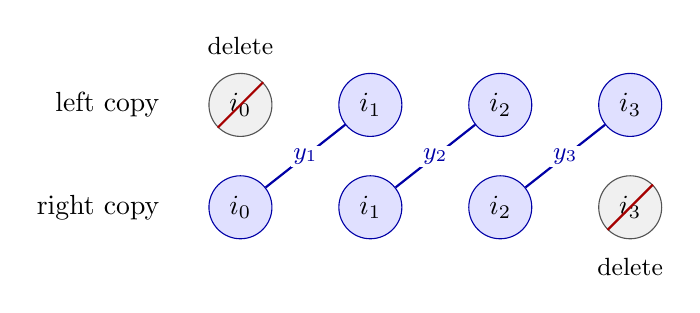
\begin{tikzpicture}[x=1.65cm,y=1.3cm,>=Latex,
 particle/.style={circle,draw,minimum size=8mm,inner sep=1pt},
 made/.style={particle,fill=blue!12,draw=blue!65!black},
 tag/.style={particle,fill=gray!12,draw=gray!65!black}]
\node[anchor=east] at (-.55,1) {left copy};
\node[anchor=east] at (-.55,0) {right copy};
\foreach \k in {0,...,3}{
 \ifnum\k=0
   \node[tag] (L\k) at (\k,1) {$i_\k$};
 \else
   \node[made] (L\k) at (\k,1) {$i_\k$};
 \fi
 \ifnum\k=3
   \node[tag] (R\k) at (\k,0) {$i_\k$};
 \else
   \node[made] (R\k) at (\k,0) {$i_\k$};
 \fi
}
\foreach \k/\j in {1/0,2/1,3/2}{
 \draw[blue!65!black,thick] (L\k) -- node[fill=white,inner sep=1pt,font=\small] {$y_\k$} (R\j);
}
\draw[red!65!black,thick] (L0.south west)--(L0.north east);
\draw[red!65!black,thick] (R3.south west)--(R3.north east);
\node[font=\small,anchor=south] at (0,1.4) {delete};
\node[font=\small,anchor=north] at (3,-.4) {delete};
\end{tikzpicture}
\caption{Midpoint transport along a three-step label list. The left path
of $i_k$ and the right path of $i_{k-1}$ are generated with common
midpoint $y_k$. Their full paths need not agree. After deleting $i_0$
on the left and $i_3$ on the right, the displayed midpoint multisets
coincide. Unlisted paths are retained in both copies.}
\label{fig:local-transport}
\end{figure}


We calculate a lift density before estimating it.  Treat the left as
the observed copy, fix $\cD$, the tags and list, and condition on the
paths $\eta$ outside
$S=\{i_1,\ldots,i_m\}$.  Put $B_S=\prod_{l\in S}B_l$.  Let
$c_S(o;\eta)$ be the product of all individual cutoff indicators on
$S$ and all checks involving at least one label in $S$.  By
Lemma~\ref{lem:conditional-path-law}, the original conditional law is
\begin{equation}\label{eq:local-reference}
 \lambda_S(\dd o\mid\eta)
       =\frac{c_S(o;\eta)}{Z_S(\eta)}B_S(\dd o),
 \qquad Z_S(\eta)=\int c_S(o;\eta)B_S(\dd o)>0.
\end{equation}
Checks wholly outside $S$ are fixed and do not enter this formula.

The generation kernel on the changed left paths has a density
$k_S(o,\eta,z)$ with respect to $B_S(\dd z)$.  To verify this
precisely, write $B_l^y$ for the free path law of label $l$ conditional
on midpoint $y$, and $g_l$ for its Gaussian midpoint density.  A pair
with observed label $l$ and auxiliary label $l'$ has proposal measure
\begin{equation}\label{eq:local-proposal}
 \frac{\1_C(z_l(0))}{g_l(z_l(0))}
                  B_l(\dd z_l)B_{l'}^{z_l(0)}(\dd z'_{l'}).
\end{equation}
Multiplication by its success indicators and division by its success
probability describes the actual insertion kernel.  Sequential
integration of the auxiliary paths gives $k_S$.  This is a density
for the observed paths only: the paired paths have a common midpoint,
and their joint law has no density against two independent bridges.

\begin{lemma}[The centered conditional likelihood]
\label{lem:local-likelihood}
Include the second tag indicator but omit its divisor $T_{w'}$.
On admissible output paths the left likelihood is
\begin{equation}\label{eq:local-likelihood}
 L_S(z;\eta)=\int c_S(o;\eta)h_{w'i_m}(o)
                      k_S(o,\eta,z)B_S(\dd o).
\end{equation}
It obeys
\begin{equation}\label{eq:local-centering}
 F_S=L_S-h_{w'i_m},\qquad
                 \int F_S\,\dd\lambda_S(\cdot\mid\eta)=0,
\end{equation}
and
\begin{equation}\label{eq:local-likelihood-bound}
                     0\le L_S\le C_xD^{C\sqrt x}.
\end{equation}
These assertions remain valid after deleting specified outside checks
consistently from the reference, the original-path integral, and all
insertion tests and their normalizing probabilities.
\end{lemma}

\begin{proof}
Before taking the likelihood, the generated density against $B_S$
is the right side of \eqref{eq:local-likelihood} divided by $Z_S$.
The output kernel is supported on $c_S(z;\eta)=1$, where the reference
density against $B_S$ is $1/Z_S$.  Thus the normalizer cancels.
Since each generation kernel has mass one, its support also gives
\[
 \int c_S(z;\eta)L_S(z;\eta)B_S(\dd z)
       =\int c_S(o;\eta)h_{w'i_m}(o)B_S(\dd o).
\]
Division by $Z_S$ proves \eqref{eq:local-centering}.  The subtracted
indicator there is evaluated on the reference output, whereas the
indicator inside \eqref{eq:local-likelihood} is evaluated on the
integrated original path.

On $C_k$, the factor $g_{i_k}^{-1}$ in
\eqref{eq:local-proposal} is at most $CD^{Cx}$, since its distance
from the mean is absolutely bounded and $t^{-1}=x\log D$.
Every success denominator costs at most two.  Dropping unused checks,
and integrating the auxiliary conditional bridges, bounds the observed
kernel density by $(CD^{Cx})^m2^m$.  The original-path integral has
mass at most one.  Since $m=O(x^{-1/2})$, this proves
\eqref{eq:local-likelihood-bound}.

Deleting checks preserves output support in the corresponding
admissible set and only improves the insertion lower bounds.  The
same argument applies on that modified conditional fiber.  For later
integrals we also define these kernels at outside values satisfying
all individual cutoffs, even if a check wholly outside $S$ fails:
that outside-only check is ignored.  The insertion bounds hold at
these histories, and the formulas represent actual conditional
likelihoods wherever the outside reference constraints hold.
\end{proof}

\subsection{Cancellation in a fourth moment}

The likelihood for one chosen list need not be close to one.  Averaging
many possible tags and interior labels produces the needed small
error.  Conditional centering cancels terms involving an isolated
list; the terms that survive have either repeated labels or at least
two rare interactions between lists.  We make both statements precise.

For fixed tags and data, put a bar over a quantity to denote averaging
over the route and interior label choices.  We claim that, for
sufficiently small fixed $x$,
\begin{equation}\label{eq:local-centered-fourth}
 \E\left[\1_{\mathcal G_{v,w'}}
       \sum_{i\in I}\frac{h_{vi}}{T_v}
       \left|\sum_{i_m\ne i}\frac{\overline{F_S}}{T_{w'}}\right|^4
       \right]\le C_{x,j}D^{-1-1/20}.
\end{equation}
Each tag sum is restricted to the fixed enlargement of its cell and
to labels in $I$.  We first prove the conditional interaction
estimate needed to expand this fourth moment.

Fix four lists with the same first tag $i$, and let $S_a$ be their
changed sets, $1\le a\le4$.  Condition on $\cD$ and on all paths
outside $U=\bigcup_aS_a$.  Join two lists if their changed sets
intersect; the connected components are called blocks.  A singleton
block contains one list, not necessarily one label.  Distinct blocks
have disjoint label sets.  Introduce a switch
$\sigma_e\in\{0,1\}$ for each unordered pair $e$ of blocks.
Turning it off deletes all checks between those blocks from the
following three places:
\begin{enumerate}
\item the union reference on $U$;
\item the original-path indicators in each likelihood integral;
\item the insertion indicators and their success probabilities.
\end{enumerate}
In the last two places, paths outside a given changed set are the
reference paths.  All individual cutoffs are retained.  The unchanged
left path of the common tag $i$ is outside every block, so checks
against it are never switched.  A newly generated right path with
label $i$, however, belongs to its generating block; its checks
against other blocks are switched.  It is never checked against the
left copy of the same label.  These rules also specify the switches
when two lists overlap.

Let $c_U^\sigma$ denote the switched union indicator and
$F_a^\sigma$ the switched centered likelihood.  Define the
unnormalized integral
\begin{equation}\label{eq:local-switch-integral}
 G(\sigma)=\int c_U^\sigma(z)
                   \prod_{a=1}^4F_a^\sigma(z)B_U(\dd z).
\end{equation}
The conditional fourth-moment summand before switching is
$G(\boldsymbol1)/Z_U$, where $Z_U=\int c_U^{\boldsymbol1}\dd B_U$.
We hold this denominator fixed throughout the switch expansion.
Successive single-path insertions give $Z_U^{-1}\le C_x$, because
$U$ has at most $4C_x$ labels.

For a block-pair edge $e$, let $\mathcal Q_e$ be the finite list of
distinct-label pairs whose checks are controlled by that switch.
It includes checks using generated auxiliary paths and original
paths, with bounded multiplicity.  All its labels and endpoints are
fixed by the data and the four lists.

\begin{lemma}[One and two switched interactions]
\label{lem:local-switches}
Suppose the four changed sets are either pairwise disjoint, or have
exactly one independent label identification.  Write $\Delta_e$ for
the finite difference from $\sigma_e=0$ to $\sigma_e=1$.  Uniformly
in all other switch settings,
\begin{equation}\label{eq:local-one-switch}
 \frac{|\Delta_eG|}{Z_U}
       \le C_xD^{C\sqrt x}\sum_{(l,k)\in\mathcal Q_e}\beta_{lk}.
\end{equation}
If the changed sets are pairwise disjoint and $e\ne f$, then
\begin{equation}\label{eq:local-two-switches}
 \frac{|\Delta_e\Delta_fG|}{Z_U}
   \le C_xD^{C\sqrt x}
       \sum_{\substack{(l,k)\in\mathcal Q_e\\
                       (l',k')\in\mathcal Q_f}}
                                 \beta_{lk}\beta_{l'k'}.
\end{equation}
The sums have at most $C_x$ terms.  Moreover
$\beta_{lk}\le C_xD^{-19/100}$ for sufficiently large $D$.
\end{lemma}

\begin{proof}
Expand each centered factor as $L_S-h_{w'i_m}$, then use
\eqref{eq:local-likelihood} for each likelihood.  Each such term has
reference output bridges on $U$, a separate collection of latent
original bridges for each likelihood, and its generated auxiliary
bridges.  The original integrations remain separate even when their
output coordinates coincide.  All individual cutoff indicators
remain in place when estimating collisions.

First consider singleton blocks.  Combine the observed bridge factor
in \eqref{eq:local-proposal} with its midpoint density and auxiliary
conditional bridge.  The result is exactly the common-uniform-midpoint
pair proposal.  After unused checks and bounded success denominators
are discarded, the variables within a singleton block therefore have
a product of ordinary original bridges and these pair proposals.
If its centered factor contributes the subtracted indicator, it uses
ordinary output bridges instead.  These base measures are independent
between blocks: their cells and endpoints depend only on $\cD$.
The common midpoint inside one pair is preserved throughout.

A difference of a check indicator forces failure of one of the checks
controlled by that edge.  Failure of \eqref{eq:soft-check} requires
a collision within the interaction range $r$.  A union bound reduces
it to one of the label pairs in $\mathcal Q_e$.  Given an allowed
opponent path, integrating a plain bridge or a marginal of the
uniform-midpoint pair proposal, with its individual cutoffs retained,
costs at most $C_x\beta_{lk}$ by \eqref{eq:beta} and the
uniform-midpoint form of \eqref{eq:midpoint-cost}.

Success denominators require the same conclusion.  At fixed history
a success probability can be written using a fresh proposal $Q$ as
\[
 p(\sigma)=\int Q(\dd z)\,c(z)
                         \prod_e A_e(z)^{\sigma_e},
                  \qquad p(\sigma)\ge\tfrac12.
\]
Here $c$ contains the individual cutoffs and unswitched checks, while
$A_e$ is the product of the checks controlled by $e$ at this stage.
We use $A^0=1$ also when $A=0$.  A first difference introduces
$A_e-1$; a mixed difference introduces
$(A_e-1)(A_f-1)$.  They force the indicated one or two collisions.
The identity
\[
                 p^{-1}-q^{-1}=\frac{q-p}{pq}
\]
and its difference in a second variable bound the second reciprocal
difference by a constant times
\[
 |\Delta_e\Delta_fp|
       +\max_\sigma|\Delta_ep(\sigma)|
                       \max_\sigma|\Delta_fp(\sigma)|.
\]
The product of first differences is represented with independent
fresh proposals.  Every such proposal belongs to the block whose
denominator produced it.  The lower bound for $p$ holds at all
histories under consideration, since only individual cutoffs are
required of earlier paths when unused checks are ignored.

The finite-product difference rule now bounds a first difference by
a finite sum of integrals with one forced cross-block collision,
and a second difference by ones with two specified cross-block
collisions.  Unused denominators cost only $C_x$.  With no label
identification, either end of one edge can be integrated as a
singleton.  For two distinct edges, their graph consists of a
two-edge tree or two disjoint edges.  In the tree case fix all
variables at the central vertex and integrate its two leaves in
succession.  Each leaf participates in one forced collision, so these
integrations give the two $\beta$ factors.  No independence between
the two collision events at the central block is required.  For
disjoint edges the two integrations are separate.  Fresh proposals
from denominator differences obey the same argument after assigning
them to their generating blocks.

With one independent identification the block sizes are $2,1,1$.
Every edge has a singleton end, which supplies the collision factor
in \eqref{eq:local-one-switch}.  After integrating that singleton,
the remaining repeated output coordinates in the block of size two
are bounded by the observed density estimate
\eqref{eq:local-likelihood-bound}: bound any surplus factors
$g_l^{-1}\1_C$ by $CD^{Cx}$ and integrate auxiliary conditional
bridges.  Across the four lists this costs at most
$C_xD^{C\sqrt x}$.  The same harmless bound covers all remaining
factors in the disjoint case.  This proves both difference estimates.
The argument allows arbitrary settings of unused switches; additional
differences are bounded by finite sums of these estimates at those
settings.  Finally \eqref{eq:beta} gives
$\beta_{lk}\le b_D(1+2/s_1)\le C_xD^{-19/100}$.
\end{proof}

We can now prove \eqref{eq:local-centered-fourth}.  Expanding the
fourth power gives four independently chosen lists, conditional on
the common first tag and the data.  There are at most $C_xDf_0$
candidates for each tag or interior slot, by the good endpoint
counts and the tube restriction.  A normalized tag counting weight
and every interior-choice probability are at most $C_{x,j}/(Df_0)$.
Split the sums by the tag mean-sites and the route site patterns;
there are only $C_x$ patterns.  We retain the original weights in
each subsum, without conditioning on a pattern and renormalizing.

An equality pattern with $q$ independent identifications has $q$
fewer free label choices.  Dominating all slot weights by their
point bounds and counting the remaining choices gives total weight
at most $C_{x,j}(Df_0)^{-q}$.  A triple equality counts as two
identifications.  These are joint counting estimates; they assert
no point-mass bound conditional on the occurrence of a coincidence.
There are only $C_x$ equality patterns.  Consequently all patterns
with $q\ge2$ contribute, by \eqref{eq:local-likelihood-bound}, at most
\begin{equation}\label{eq:local-many-identifications}
                         C_{x,j}D^{-2+2x+C\sqrt x}.
\end{equation}

For $q=0$ or $1$, use the switches above.  For an edge set $E$, let
$\Delta_E=\prod_{e\in E}\Delta_e$.  The elementary Boolean identity is
\begin{equation}\label{eq:local-boolean}
                   G(\boldsymbol1)=\sum_E\Delta_EG(\boldsymbol0).
\end{equation}
If the graph with edge set $E$ has an isolated singleton block, its
term vanishes.  Indeed all edges from that block are off in every
evaluation comprising the difference.  Its variables separate from
the others, and their integral is
\[
                       \int c_S F_S\,\dd B_S=0
\]
by \eqref{eq:local-centering}.  This is why the common denominator
$Z_U$ was held fixed rather than switched.

When $q=1$ there are three blocks, two of them singletons, so a
nonzero term must contain an edge.  Its identification cost and
\eqref{eq:local-one-switch} give total contribution at most
\begin{equation}\label{eq:local-one-identification}
                    C_{x,j}D^{-1+x-19/100+C\sqrt x}.
\end{equation}
When $q=0$, all four blocks are singletons and a nonzero term has
at least two distinct edges.  Apply \eqref{eq:local-two-switches}
to any two of them, and bound any remaining differences by a finite
sum of evaluations with the other switches fixed.

One of these two collision factors can be averaged over a label
slot.  Every cross-block check has at least one label in a changed
set, whereas the common tag $i$ belongs to none of those sets.
The endpoint bound \eqref{eq:flag-count}, summed over dyadic annuli
in a fixed neighborhood, gives uniformly in the other endpoint $y$
\begin{equation}\label{eq:label-average}
 \frac{C_{x,j}}{Df_0}
       \sum_{k\text{ in a slot range}}
                 \frac1{s_1\vee d_K(y,Y_k)}
 \le C_{x,j}\left(1+\frac{D^{1/100}}{Df_0s_1}\right)
 \le C_{x,j}.
\end{equation}
For example, a dyadic annulus of radius $h\le1$ contributes at most
$C_{x,j}(h^2+D^{1/100}/(Df_0h))$; the innermost ball is bounded at
radius $s_1$, and the unit-scale and larger annuli use the unit-count
bound.  The geometric sums give the displayed expression.  The same
estimate holds with $Z_k$ in place of $Y_k$.  Thus averaging this
factor costs at most $C_{x,j}b_D$.  Bound the other factor by
$C_xD^{-19/100}$.  In these positive bounds we may remove all further
noncoincidence restrictions and enlarge the label sums.  The total
contribution with no identification is therefore at most
\begin{equation}\label{eq:local-no-identification}
                    C_{x,j}D^{-19/100+C\sqrt x}b_D.
\end{equation}
The first-tag factor $h_{vi}$ is fixed in every conditional integral,
so it does not disturb centering.  Its total normalized tag sum on
good data is bounded by $C_{x,j}$.  Equations
\eqref{eq:local-many-identifications}--\eqref{eq:local-no-identification}
prove \eqref{eq:local-centered-fourth} once $x$ is chosen sufficiently
small.  Indeed $b_D=C_xD^{-1}(\log D)^C$, and all three powers then
save more than $1/20$ beyond $D^{-1}$.

\subsection{The local comparison after projection}

Let $\ell_v$ and $\ell_{w'}$ be the two lifted densities of
$\nu_{v,w'}$ relative to their augmented references.  On retained
data with first tag in $I$, the left density is
\[
                  \ell_v=\sum_{i_m\ne i}\frac{\overline{L_S}}{T_{w'}};
\]
set it to zero on the omitted part of the reference.  The centered
subtraction sums to $A_{w'}-M_{w'}'$.  In fact the candidate mean
range contains every tag with nonzero $h_{w'i_m}$, by confinement,
and the excluded first tag has $h_{w'i}=0$ because the cells are
disjoint.  Thus on the retained part
\begin{equation}\label{eq:local-lift-error}
 \ell_v-1=\sum_{i_m\ne i}\frac{\overline{F_S}}{T_{w'}}
                              +(A_{w'}-1)-M_{w'}'.
\end{equation}

\begin{proposition}[Adjacent deletion measures]\label{prop:local-palm}
For sufficiently small fixed $x>0$, depending on $u$, the common
measure constructed above satisfies
\begin{equation}\label{eq:local-lift-fourth}
 \E_{v\sim w'}\left[
       \int|\ell_v-1|^4\,\dd P_{\mathrm{aug},v}
       +\int|\ell_{w'}-1|^4\,\dd P_{\mathrm{aug},w'}\right]
                         \le C_jD^{-1-u/8}.
\end{equation}
Consequently the local comparison~\eqref{eq:local-fourth} holds.
That bound, with a fixed change of constant, also holds when only
adjacent pairs inside the same $R$-cell are retained in the average.
\end{proposition}

\begin{proof}
Apply $|a+b+c|^4\le27(|a|^4+|b|^4+|c|^4)$ to
\eqref{eq:local-lift-error}.  The centered term is controlled by
\eqref{eq:local-centered-fourth}.  Off the negligible count tail,
the count-fluctuation term is at most
\[
 \E[A_v|A_{w'}-1|^4]
     \le C_jD^x\E|A_{w'}-1|^4+O(D^{-A})
\]
for any prescribed fixed $A$.  Averaging adjacent cells and using
\eqref{eq:flag-moments} bounds it by
$C_j(D^{-1-u/6+x}+D^{-2+3x})$.  Likewise,
\[
 \E[A_v(M_{w'}')^4]
       \le C_jD^{4x}\E M_{w'}'+O(D^{-A})
       \le C_{x,j}D^{-1-1/8+4x}+O(D^{-A}).
\]
The part where $\ell_v$ was set to zero contributes its reference
mass, controlled by \eqref{eq:tag-omission} and
\eqref{eq:good-omission}.  Taking $x<u/24$ in addition to the earlier
smallness conditions makes all these terms bounded by
$C_jD^{-1-u/8}$.

For the right lift, regard the right copy as observed, reverse the
list indices, and keep the actual generation order.  Its unchanged
tag is now $i_m$ and its changed set excludes $i_m$.  The density
formula, switched centering, and collision integrations are unchanged:
they allow any fixed insertion order.  This proves
\eqref{eq:local-lift-fourth} for the two lifts of the same measure.

Under a measurable projection, the projected likelihood is the
conditional expectation of the lifted likelihood.  Conditional
Jensen therefore transfers each fourth-moment bound to the density
of $\nu_{v,w'}$ relative to $P_v$ or $P_{w'}$.  Write $q(Y')$ for
its Lebesgue density and put $y=s_v(Y')$, $z=s_{w'}(Y')$.
Absolute continuity with respect to both references makes $q=0$
where either reference density vanishes.  Inserting $\sqrt q$ between
$y$ and $z$, and using $|1-\sqrt a|\le|1-a|$ for $a\ge0$, gives
\[
 \frac{|y-z|^4}{y^2+z^2}
   \le 8\left[y^2\left|1-\frac q{y^2}\right|^4
               +z^2\left|1-\frac q{z^2}\right|^4\right].
\]
Terms with zero prefactor are omitted.  Integrating this inequality
and applying the two projected bounds proves \eqref{eq:local-fourth}.
Restricting the nonnegative edge sum to edges within $R$-cells only
decreases it; the normalizations differ by a bounded factor.
\end{proof}

\section{Distant deletion comparisons}\label{sec:long-palm}

We now compare the deletion measures for distant cells of side $R$.
We prove \eqref{eq:distant-comparison} for the ordered $R$-cell pairs
$\mathcal P_R$ defined at the beginning of Section~\ref{sec:paths}.
The local construction of Section~\ref{sec:local-palm} cannot simply be
iterated: its route would have length growing with $K$, whereas even a
fixed loss at each step would destroy the estimate.  We instead retain
the original paths near both ends of a long random route.  In a product
of two likelihoods, the resulting errors occur only when the changed
portions of the two routes meet.  A geometric input makes these meetings
rare and controls their number exponentially.

\subsection{The geometric input and its application}

We use the following complete statement of \cite[Proposition~7.1]{D}.
It concerns a random set of lattice sites only.  The proof in
\cite[Section~7]{D} uses folded paths and the unpredictable-path
method of \cite{BPP}.

\begin{proposition}[Routes with rare encounters away from the common end]
\label{prop:route-input}
On $\mathcal L_K=(\Z/K\Z)^3$, let $d_\infty$ be the periodic maximum
distance.  A random datum $\mathcal D$ determines a bad set
$\mathcal B\subset\mathcal L_K$ satisfying
\[
 \Pp(A\subset\mathcal B)\le p^{|A|}\qquad(A\subset\mathcal L_K).
\]
Fix an integer contact radius $r_c\ge1$, an integer $q\ge0$, and $c_Q>0$.
Let $Q$ be a projected lattice cube of side at most $c_QR$, and let
$z$ be a site such that every $y\in Q$ has forward first-coordinate
displacement from $z$ in $[.29K,.46K]$.  There are constants
$p_0,\kappa,c,C,C_0>0$ and $R_0$, depending only on the fixed
parameters, with the following properties when $R\ge R_0$,
$K\ge C_0R$, and $p\le p_0$.

Put $H=\lfloor R^{1/2}\rfloor$.  There is an event $\mathcal E$,
determined by $\mathcal D,z,Q$, on which one can sample simple good
nearest-neighbor routes $\pi_y$ from $z$ to every $y\in Q$.
Conditional on $\mathcal D$, different samples use independent fresh
randomness.  The event $\mathcal E$ includes the requirement that the
$10R$-neighborhoods of $z$ and $Q$ contain no bad sites.

For $\pi=(v_0,\ldots,v_m)$ starting at $z$, put
\[
 a(\pi)=\max\{i:d_\infty(v_i,z)\le H\},\qquad
 \pi^{\rm ch}=\{v_i:i>a(\pi)\}.
\]
The initial portion $(v_0,\ldots,v_{a(\pi)})$ has at most $CH$
vertices.  The analogous portion read backwards from the terminal
site also has at most $CH$ vertices, and these two portions are
disjoint.  Let $\pi^{\rm ch,q}$ contain the vertices whose path index
is within $q$ of an index in $\pi^{\rm ch}$.  For independent samples
$\pi_y,\pi_{y'}$, set
\[
 J_c=\sum_{v\in\pi_y}\sum_{v'\in\pi_{y'}}
       \1_{\{d_\infty(v,v')\le r_c\}},\qquad
 J_*=\sum_{v\in\pi_y^{\rm ch,q}}
       \sum_{v'\in\pi_{y'}^{\rm ch,q}}
       \1_{\{d_\infty(v,v')\le r_c\}}.
\]
Uniformly in the specified endpoints,
\begin{equation}\label{eq:route-exponential}
 \E_{\mathcal D}\bigl[\1_{\mathcal E}
       \E_{\rm routes}(e^{\kappa J_c}\mid\mathcal D)\bigr]\le C.
\end{equation}
For every deterministic probability mass function $\omega$ on
$Q\times Q$ with $\omega(y,y')\le C_\omega R^{-6}$,
\begin{equation}\label{eq:route-rare}
 \sum_{y,y'\in Q}\omega(y,y')
   \E_{\mathcal D}\bigl[\1_{\mathcal E}
       \Pp_{\rm routes}(J_*>0\mid\mathcal D)\bigr]
 \le CC_\omega R^{-c_g},\qquad
 c_g=\frac12\left(\frac{\log2}{\log3}-\frac12\right)>0.
\end{equation}
Both estimates hold with a common terminal endpoint, reading the same
route construction in reverse order.  Finally, if $\mathcal M$ is
the stated bad-free margin event, then
\begin{equation}\label{eq:route-rejection}
 \Pp(\mathcal M\setminus\mathcal E)
 \le K^3(Ap)^{\lfloor K/(10(r_c+2))\rfloor}+CR^3e^{-cR},
\end{equation}
where $A$ is fixed and $Ap_0<1$.
\end{proposition}

We check the hypotheses and fix how this result is used.  The bad sites
are those of Section~\ref{sec:paths}.  Equation~\eqref{eq:good-prob}
gives the required joint bound with any sufficiently small fixed $p$,
by increasing the threshold for $D$.  All possible mean-sites of tags
whose midpoint lies in $v$ belong to a fixed enlargement $Q_v$ of that
cell, of side $O_x(R)$; this follows from the individual tubes.  The
same holds for $w'$.  Since $K/R\to\infty$ in the thermodynamic limit,
the displacements from any site of $Q_v$ to any site of $Q_{w'}$
belong to the wider interval in Proposition~\ref{prop:route-input}.

Choose $r_c$ large enough, in terms of $b_0$, to contain every possible
cross-route interaction between paths in their individual tubes, as
well as the bounded offsets between sites and means.  Take $q=2$ to
allow the adjacent labels used by a paired insertion.  These choices
are fixed once $x$ is fixed.  We retain a bad-free margin of radius
$C_xR$ around both cells and impose the route-availability events for
every endpoint site in their enlarged cubes, for both orientations.
There are only polynomially many such sites in $R$.  Thus
\eqref{eq:route-rejection} bounds the additional rejection by
$o_K(1)+C_xR^{C_x}e^{-c_xR}$.  This extra retention can only decrease
the nonnegative quantities in
\eqref{eq:route-exponential}--\eqref{eq:route-rare}.

We always sample the routes by the construction of
Proposition~\ref{prop:route-input}, conditional on the datum and the
endpoint sites.  In a likelihood product, the datum is shared and the
route randomizations are independent.  In particular, we do not
condition their law on a subsequent successful path insertion.
The exponent $c_g$ is independent of $x$, although the constants and
$\kappa$ may depend on $x$.

\subsection{A common measure with retained end portions}

Use the tag weight \eqref{eq:tag-pair-weight} for $(v,w')\in\mathcal P_R$,
retained data, and distinct tags $i_0,i_m\in I$.  On the sampled route
from their mean-sites choose one interior label at each intermediate
site, uniformly and independently given the tags and sites, excluding
the two tags.  The resulting list $i_0,\ldots,i_m$ has distinct labels;
each interior choice has atom at most $C_x/(Df_0)$.  Successive means
are at bounded absolute distance.

Write the initial silent portion of the route as $k<a_0$, and its
terminal silent portion as $k>a_1$.  Thus $a_0$ is one plus the last
visit within distance $H$ of the initial site, while $a_1$ is one less
than the first index in the terminal portion.  Both tags lie in these
portions, and the portions are disjoint.  Keep all unlisted paths in
both copies.  Keep the prefix originals $k<a_0$ on the left, and the
suffix originals $k>a_1$ on the right.  The remaining paths are
generated as follows, pairing left label $i_k$ with right label
$i_{k-1}$ for $1\le k\le m$.

\begin{enumerate}
\item For $a_0\le k\le a_1+1$, propose a common uniform midpoint
in a unit cell within bounded distance of both means and propose the
two paths independently conditional on that midpoint.  Condition
jointly on their individual cutoffs, the checks
\eqref{eq:soft-check} against retained and previously generated paths
in their respective copies, and midpoint separation by $s_1$ from
those opponents.  These middle pairs are probability kernels:
Proposition~\ref{prop:insertion}, Assertion~2, bounds each success
probability below by $1/2$.  Use any fixed order for them.

\item In every other pair, one path is a retained original.  Pin the
other path to its midpoint $y$.  Give this step mass zero unless $y$
is within $8b_0$ of the new label's mean and is $s_1$-separated from
all opponent midpoints already present in the copy receiving the
new path.  If these conditions hold, propose the bridge pinned at
$y$, impose its individual cutoffs and checks
\eqref{eq:soft-check}, and divide by
\begin{equation}\label{eq:pin-denominator}
 \max\{1/2,p_{\rm pin}\},
\end{equation}
where $p_{\rm pin}$ is their success probability under the pinned
proposal.  This is a subprobability kernel.  Perform these steps
after all middle pairs, in fixed orders.  Prefix pins are inserted
on the right and suffix pins on the left; neither family uses paths
generated by the other family.
\end{enumerate}

The final copies satisfy all conditional reference checks.  Every
left midpoint except that of $i_0$ agrees with its paired right
midpoint, and every right midpoint except that of $i_m$ is paired.
Deleting these respective tags and using the common ordering of the
bath coordinates therefore gives one measure on the bath with lifts
to both augmented references.  Figure~\ref{fig:silent-transport}
shows the pairing and the retained end portions.

\begin{figure}[tb]
\centering
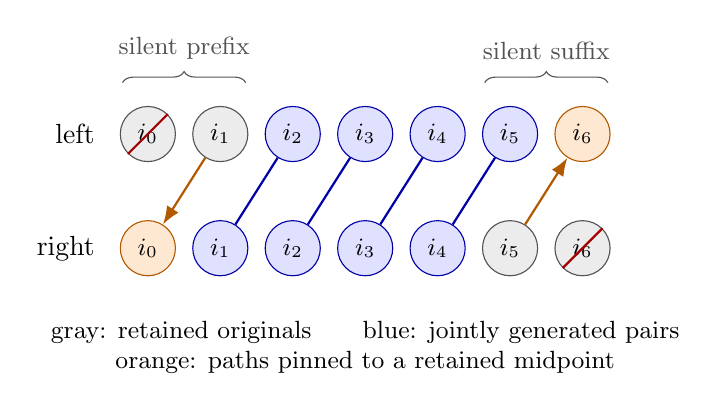
\begin{tikzpicture}[x=.92cm,y=1.45cm,>=Latex,
 particle/.style={circle,draw,minimum size=7mm,inner sep=1pt,font=\small},
 made/.style={particle,fill=blue!12,draw=blue!65!black},
 pinned/.style={particle,fill=orange!18,draw=orange!70!black},
 old/.style={particle,fill=gray!15,draw=gray!65!black}]
\node[anchor=east] at (-.6,1) {left};
\node[anchor=east] at (-.6,0) {right};
\foreach \k in {0,1}{\node[old] (L\k) at (\k,1) {$i_\k$};}
\foreach \k in {2,3,4,5}{\node[made] (L\k) at (\k,1) {$i_\k$};}
\node[pinned] (L6) at (6,1) {$i_6$};
\node[pinned] (R0) at (0,0) {$i_0$};
\foreach \k in {1,2,3,4}{\node[made] (R\k) at (\k,0) {$i_\k$};}
\foreach \k in {5,6}{\node[old] (R\k) at (\k,0) {$i_\k$};}
\foreach \k/\j in {2/1,3/2,4/3,5/4}{\draw[blue!65!black,thick] (L\k)--(R\j);}
\draw[orange!70!black,thick,->] (L1)--(R0);
\draw[orange!70!black,thick,->] (R5)--(L6);
\draw[red!65!black,thick] (L0.south west)--(L0.north east);
\draw[red!65!black,thick] (R6.south west)--(R6.north east);
\draw[decorate,decoration={brace,amplitude=4pt},gray!65!black]
 (-.35,1.45)--(1.35,1.45) node[midway,above=5pt,font=\small] {silent prefix};
\draw[decorate,decoration={brace,amplitude=4pt},gray!65!black]
 (4.65,1.45)--(6.35,1.45) node[midway,above=5pt,font=\small] {silent suffix};
\node[anchor=north,font=\small,align=center] at (3,-.55)
 {gray: retained originals\qquad blue: jointly generated pairs\\
 orange: paths pinned to a retained midpoint};
\end{tikzpicture}
\caption{A schematic long comparison with $a_0=2$ and $a_1=4$.
The left prefix and right suffix retain their original paths. Central
pairs receive common proposed midpoints; an end pin copies the midpoint
of its retained partner in the other copy. The arrows indicate the
source of a pin, not equality of full paths. The changed left set is
$\{i_2,\ldots,i_6\}$, which excludes the common first tag. Deleting the
crossed tags again leaves identical midpoint multisets.}
\label{fig:silent-transport}
\end{figure}


The silent portions have two purposes.  They keep the common tag
outside the changed set in a likelihood product, and they ensure that
the changed sets start far enough from their common end for
\eqref{eq:route-rare} to apply.  The opposite-copy pins preserve the
matching of bath midpoints across these retained portions.

\begin{lemma}\label{lem:long-mass}
The common measure just constructed has mass satisfying
\begin{equation}\label{eq:long-mass}
 \operatorname{mass}\ge \E[A_vA_{w'}]-CD^{-1-c'}-o_K(1)
\end{equation}
for some $c'>0$ and sufficiently small fixed $w,x$.
\end{lemma}
\begin{proof}
The tag omissions, the bad-free margins, and the route rejections
have the stated cost by \eqref{eq:good-prob},
\eqref{eq:tag-omission}, and \eqref{eq:route-rejection}; the margins
contain $O_x(R^3)$ sites, and extra relative count factors cost only
fixed powers $D^x$, apart from negligible count tails.  Impose also
the full-path bounds of Section~\ref{sec:paths} on the original
sample in the endpoint neighborhoods of radius $O_x(R)$.  Their
failure has smaller cost, by the last line of
\eqref{eq:good-prob}.  This event is used only to estimate the mass;
we do not condition the reference bridges on it.

On this original-sample event, all pins lie in range: the retained
original has displacement at most $b_0$ from its endpoints, and
successive means are at bounded distance.  Whenever the required
midpoint separations hold, every $p_{\rm pin}\ge3/4$ by
Proposition~\ref{prop:insertion}, Assertion~3.  Indeed its opponents
are the original collection, with some originals deleted and some
generated paths added.  Route simplicity and the individual tubes
bound the number of added paths relevant to any fixed neighborhood
independently of the route length.  Consequently all such pin
kernels have mass one.

Separation from a middle path was already imposed when that middle
pair was generated: in the other copy its common midpoint was
tested against the retained original which supplies the pin.  The
two silent ends are far apart.  Every remaining separation failure
therefore entails two original midpoints at distance at most $s_1$
in an endpoint neighborhood.  Equation~\eqref{eq:pair-bound} bounds
their expected ordered count in each fixed site neighborhood by
$C_xD^2s_1^3$.

The choice of an interior label has atom at most $C_x/(Df_0)$ even
after fixing the data and tags.  A route visits a site at most once,
so we can sum this bound over all endpoint neighborhoods, of total
volume $O_x(R^3)$, without conditioning any count on route
availability.  A tag appearing in such a test supplies at least the
same weight through its divisor.  The other tag factors are bounded
by relative counts.  More explicitly, restrict all unit counts in
these neighborhoods to $CD$; by
\eqref{eq:count-tails}--\eqref{eq:count-mgf}, the discarded parts
contribute less than every inverse power of $D$, even after fixed
count products and polynomially many site sums.  The remaining loss
is at most
\[
 C_xR^3D^{Cx}\frac{D^2s_1^3}{Df_0}.
\]
Since $D^2s_1^3=D^{-2/5}$ and $R\asymp D^w$, this is
$O(D^{-1-c'})$ for sufficiently small $w,x$.  Middle steps never
lose mass.  Summing the tag weights proves \eqref{eq:long-mass}.
\end{proof}

\subsection{Conditional likelihoods and removal of cross checks}

We next bound the second moment of a lift.  Unlike a uniform bound
on its density, this estimate will have no factor depending on route
length.  Treat the left copy as the observed, or primary, copy.  Its
changed labels form
\[
 S=\{i_k:k\ge a_0\}.
\]
Fix the datum, tags, route and list, and condition on the paths $o$
outside $S$.  With $B_S$ the product plain bridge law and $c_S$ the
conditional reference indicator, write
\begin{equation}\label{eq:long-kernel}
 M_S(o;\dd z)=\int c_S(y;o)h_{w'i_m}(y)
                    K_S(y,o;\dd z)\,B_S(\dd y),\qquad
 Z_S(o)=\int c_S(y;o)\,B_S(\dd y).
\end{equation}
Here $y$ denotes latent original paths, $z$ the primary outputs,
and $K_S$ the subprobability kernel of all generation steps.  The
likelihood, before the divisor $T_{w'}$, is
$L_S=\dd M_S/\dd B_S$ on admissible reference outputs: the input
and output conditional normalizer $Z_S$ cancels exactly.  Absolute
continuity is verified below, including for the pins.

For an upper bound we may integrate out the pins generated on the
right at the silent prefix and replace their total mass by one.
No primary middle or pin step uses those paths.  We use the same
notation $M_S$ for this enlarged measure when taking upper bounds.

Take a second, independently sampled route and list with the same
first tag $i_0=i$.  Denote its changed set by $T$ and the two terminal
tags by $j_1,j_2$.  Condition now on all paths outside $U=S\cup T$,
as well as the datum.  In the $S$ construction remove all checks
against outside labels in $T\setminus S$, both from the latent
reference and from every proposal and success normalization.
In the $T$ construction remove checks against $S\setminus T$.
Write $A_S^-,Z_S^-,M_S^-$ for the resulting reference indicator,
normalizer, and unnormalized output measure, and similarly for $T$.
These two constructions now use only their own latent and generated
variables and the fixed paths outside $U$.

This independence also holds at the edge of a silent prefix.  Its
right pins have been integrated out.  If an old prefix path is
removed as an outside obstacle, no other part of the construction
uses that trajectory.  A right middle partner uses the fixed
endpoints of its label, not its old trajectory.  Routes and label
choices use only data, sites, and tag identities, all fixed here.

Let $Z_U=\int c_U\,\dd B_U$ be the union reference normalizer.
List all checks affected by the removals: reference checks and
checks of latent or generated paths against removed old obstacles,
including those in the success probabilities.  Every such check
requires two route vertices within $r_c$, allowing the fixed step
offsets in $J_*$.  There are at most $C_xJ_*$ such checks, with
bounded multiplicity.  The simplicity of each route gives this
bound regardless of its length.  Only distinct-label checks are
listed; in particular, a proposal never gains a check against its
own old trajectory if that trajectory was not an obstacle originally.

Let $B_{ST}$ be the sum, with these bounded multiplicities, of the
corresponding costs $\beta_{lk}$ from \eqref{eq:beta}.  For pin checks
also sum their costs $m(y,\omega)$ from
\eqref{eq:midpoint-cost}, writing the result as $M_{ST}'$.
The first quantity depends on the fixed endpoints and labels; the
second can depend on latent or generated midpoints.  Uniformly,
\begin{equation}\label{eq:cross-check-cost}
 B_{ST}+M_{ST}'\le C_xD^{-.19}J_c.
\end{equation}

The following estimate is the aim of the conditional comparison.  For
disjoint changed sets it preserves the original tag product, with an
error charged only to cross-route checks.  For overlapping sets it
charges a density bound only to the shared output labels.  Put
$G_D=C_xD^{C\sqrt x}$, with the constants sufficiently large.

\begin{lemma}[Conditional product bound]\label{lem:long-product}
Conditional on $\mathcal D$ and the paths outside $U=S\cup T$,
the two likelihoods satisfy
\begin{align}
 S\cap T=\varnothing:\quad
 \E[L_SL_T\mid U^c]
 &\le \E[h_{w'j_1}h_{w'j_2}\mid U^c]
   +Ce^{C_xD^{-.19}J_c}
       \bigl(B_{ST}+C_xJ_*b_D(1+t^{-3/2})\bigr),
       \label{eq:long-product}\\
 |S\cap T|=q\ge1:\quad
 \E[L_SL_T\mid U^c]
 &\le e^{C_xD^{-.19}J_c}G_D^q.
       \label{eq:long-product-overlap}
\end{align}
\end{lemma}

We prove the lemma through three comparisons: first of the reference
normalizers, then of the generation kernels when cross checks are
removed, and finally of the primary output densities on shared labels.

\begin{lemma}\label{lem:normalizer-comparison}
For these conditional reference laws,
\begin{equation}\label{eq:long-normalizer}
 \frac{Z_S^-Z_T^-}{Z_U}
       \le C^{|S\cap T|}e^{CB_{ST}}.
\end{equation}
If $S\cap T=\varnothing$, then for any measurable $0\le F\le1$
of the latent originals,
\begin{equation}\label{eq:reference-difference}
 0\le \frac1{Z_U}\int F(A_S^-A_T^--c_U)\,\dd B_U
          \le CB_{ST}e^{CB_{ST}}.
\end{equation}
\end{lemma}
\begin{proof}
For disjoint sets, $Z_S^-Z_T^-$ is the reference integral with
the cross checks removed.  Add these checks one at a time.
Conditional single-label insertion gives density domination by a
constant times the corresponding plain bridge, uniformly with any
subset of checks retained.  A newly added check therefore fails
with probability at most $C\beta_{lk}$.  Since the maximum of these
costs tends to zero, the loss of normalizer is at most
$e^{C\beta_{lk}}$ at that step.  Multiplication proves
\eqref{eq:long-normalizer} in the disjoint case.  Summing the
integrals lost when the checks are restored gives
\eqref{eq:reference-difference}.  All normalizers are positive by
successive insertion; no lower bound uniform in the number of
labels is being used.

If $q=|S\cap T|>0$, first delete the shared labels from both
separate integrals, which increases them because the integrands
are indicators.  Compare the remaining disjoint integrals as
above.  Insert the $q$ shared labels into the union reference,
one at a time; each insertion costs at most a fixed inverse
success probability.  Their total expense is $C^q$, proving
\eqref{eq:long-normalizer}.
\end{proof}

There is also a comparison before any generated variables are
integrated.  The original two constructions are dominated by the
separate constructions times a factor bounded in both forms
\begin{equation}\label{eq:protocol-comparison}
 e^{C_xD^{-.19}J_c},\qquad
 1+Ce^{C_xD^{-.19}J_c}(B_{ST}+M_{ST}').
\end{equation}
To prove this, fix a history at an affected transition.  Removing
checks increases its success probability from $p$ to $p^-$.  For a
middle step $p\ge1/2$; for a pin the denominator is the function
$\max(1/2,p)$, which is Lipschitz and bounded below by $1/2$.
Thus the expense in the likelihood density is at most
\[
 \frac{\max(1/2,p^-)}{\max(1/2,p)}\le1+2(p^--p),
\]
with the same estimate for the uncapped middle denominators.  Removing the preliminary pin-separation indicator
only enlarges the integrand.  For a middle step, integrate the
removed checks against its common uniform midpoint proposal;
Proposition~\ref{prop:insertion} bounds the difference by the sum
of $C\beta_{lk}$, including failures of midpoint separation.  For
a pin step the same bound includes its costs
\eqref{eq:midpoint-cost}; the needed midpoint separation holds
on the support of the old integrand.  Products of these bounds,
and \eqref{eq:cross-check-cost}, prove
\eqref{eq:protocol-comparison}.  Indicators of fewer reference
checks only enlarge an integrand.  Every unaffected transition
has ratio exactly one.

\subsection{Primary output densities and the conditional product bound}

We need one density estimate when two changed sets share labels.
For any $q$ specified primary labels, the marginal of $M_S^-/Z_S^-$
has density at most
\begin{equation}\label{eq:primary-density}
 G_D^q\quad\hbox{against their product plain bridges}.
\end{equation}
To prove it, omit the terminal tag indicator, so the latent originals
have their normalized separate reference law.  Fix those originals,
denoted by $y$, and let $K_S^-$ denote the separate generation kernel.
Divide the specified primary indices into middle indices $A_{\rm mid}$
and pin indices $A_{\rm pin}$.  A primary pin with index $k$ uses the
midpoint of the retained original label $i_{k-1}$ in the right suffix.
Write $\mathcal R_k=\{\xi:|\xi-m_{i_k}|\le8b_0\}$ for its pin range
in the compatible lift.

Conditional on the generation history, a specified middle output
is bounded by $C_xD^{Cx}B_{i_k}$, by
\eqref{eq:local-proposal}.  A specified pin is bounded by
$2\1_{\mathcal R_k}(y_{i_{k-1}}(0))
B_{i_k}^{y_{i_{k-1}}(0)}$, where the superscript denotes a prescribed
midpoint.  These majorants no longer depend on earlier generated
paths.  Integrating the generation steps in reverse order against
a nonnegative test of the specified outputs therefore gives the
conditional marginal bound
\begin{equation}\label{eq:primary-conditional-majorant}
\begin{split}
 K_S^-(y,o;\dd z_A)\le{}&
 (C_xD^{Cx})^{|A_{\rm mid}|}2^{|A_{\rm pin}|}
 \prod_{k\in A_{\rm mid}}B_{i_k}(\dd z_k)\\
 &\times\prod_{k\in A_{\rm pin}}
 \1_{\mathcal R_k}(y_{i_{k-1}}(0))
 B_{i_k}^{y_{i_{k-1}}(0)}(\dd z_k).
\end{split}
\end{equation}
Here $A=A_{\rm mid}\cup A_{\rm pin}$, and $z_k$ denotes the primary
output path of label $i_k$.  Every unspecified step contributes at
most its mass, which is at most one.  Thus the displayed product
bound does not require independence of the accepted outputs.

The sources $i_{k-1}$ of the specified pins are distinct latent labels
in $S$.  Corollary~\ref{cor:bridge-domination} bounds their joint
latent marginal by $C^{|A_{\rm pin}|}$ times their product plain
bridges.  Keep their confinement indicators when making this
comparison, so all source midpoints use the chosen local lifts.
Dropping the remaining source cutoffs in those lifts only enlarges
the integral.  For a source $l=i_{k-1}$, evaluate the resulting
midpoint mixture by the measure identity
\begin{equation}\label{eq:pin-mixture-density}
 \int_{\mathcal R_k}g_l(\xi)B_{i_k}^{\xi}(\dd z_k)\,\dd\xi
 =\1_{\mathcal R_k}(z_k(0))
   \frac{g_l(z_k(0))}{g_{i_k}(z_k(0))}
       B_{i_k}(\dd z_k).
\end{equation}
The two means are at bounded distance, and the indicator restricts
the ratio to the primary pin range.  Thus
\eqref{eq:midpoint-ratio} bounds this ratio by
$C_xD^{C\sqrt x}$.  Applying this to each pin in
\eqref{eq:primary-conditional-majorant} proves
\eqref{eq:primary-density}.  The same argument with the original
checks in place proves absolute continuity of all primary outputs
in \eqref{eq:long-kernel}.  Only the primary marginal acquires this
density; a pair with a common midpoint is still singular relative
to two independent full bridges.

\begin{proof}[Proof of Lemma~\ref{lem:long-product}]
Integrate the enlarged output measures against the common union
reference, with divisor $Z_U$, and use
\eqref{eq:protocol-comparison}.  Dropping the union output
admissibility indicator increases the resulting nonnegative
integrals.

First suppose $S,T$ are disjoint.  The leading $1$ in the second
bound of \eqref{eq:protocol-comparison} contributes at most
\[
 \frac1{Z_U}\int h_{w'j_1}h_{w'j_2}A_S^-A_T^-\,\dd B_U:
\]
the two separate kernels use different outputs and have mass at
most one.  Equation~\eqref{eq:reference-difference} compares this
to the leading conditional expectation in
\eqref{eq:long-product}.  The $B_{ST}$ error is bounded with
\eqref{eq:long-normalizer}.

For a term of $M_{ST}'$, the pin midpoint belongs to a latent
source $l$ in one separate construction and is tested against an
output path $z_k$ in the other.  After the cross checks have been removed,
the two constructions have product law at the fixed outside paths.
Write $\lambda_S^-$ for the normalized separate latent reference
and $\nu_T^-=M_T^-/Z_T^-$ for the opposing output measure, of mass
at most one.  The source-side kernels also have mass at most one.
Dropping the source-side tag indicator and integrating those kernels bounds
the normalized cost by
\[
 \int \nu_T^-(\dd z)\int\lambda_S^-(\dd y)
   \frac{b_D}{s_1\vee d_K(y_l(0),z_k(0))}
 \le C\sup_{\xi}\int
   \frac{b_Dg_l(\eta)}{s_1\vee d_K(\eta,\xi)}\,\dd\eta.
\]
Here single-label insertion bounded the source midpoint marginal
by $Cg_l$ in its local lift.  For every fixed opposing midpoint
$\xi$,
\begin{equation}\label{eq:pin-cost-average}
 \int \frac{b_D}{s_1\vee d_K(\eta,\xi)}g_l(\eta)\,\dd\eta
          \le Cb_D(1+t^{-3/2}).
\end{equation}
Indeed $g_l$, or its periodization, is bounded by $Ct^{-3/2}$,
the inverse-distance function is integrable on a unit ball in
three dimensions, and outside that ball it is at most one.
There is no need to bound the density of the opposing midpoint.
There are at most $C_xJ_*$ terms.  The normalizer ratio in
\eqref{eq:long-normalizer} completes the disjoint estimate.

When $q=|S\cap T|>0$, use the exponential bound in
\eqref{eq:protocol-comparison}.  After division by $Z_S^-Z_T^-$,
the remaining integral is the product of the two normalized
separate output densities, identifying the common output
coordinates only on $S\cap T$.  Integrating the unshared outputs
leaves the product of the two marginals on these $q$ labels.
Bound one by \eqref{eq:primary-density}; the other has mass at
most one.  Equation~\eqref{eq:long-normalizer} proves
\eqref{eq:long-product-overlap}.

For clarity, these comparisons take place first between measures
on latent originals and generated proposals, with all success
indicators and denominators present.  Their domination passes
to the primary output densities.  In the disjoint estimate we
retain the latent pin source until applying
\eqref{eq:pin-cost-average}; disintegration over the absolutely
continuous primary outputs justifies this operation.  In the
overlap estimate the two latent integrations remain separate,
and density versions agree almost everywhere under the union
product bridge measure by Fubini's theorem.  At no point do we
assign a product-bridge density to a midpoint-matched pair.
\end{proof}

\subsection{Averaging the labels and route encounters}

Let $\ell_v$ be the left lift likelihood, with zero value on
omitted data and tags.  On the retained part it is the sum of
$\overline{L_S}/T_{w'}$ over second tags, where the bar averages
the route and interior label kernels.  Squaring it gives two
independent choices with common first tag $i$.  The augmented
reference supplies its factor $h_{vi}/T_v$ only once; this path
is fixed outside $U$.  The disjoint leading term in
\eqref{eq:long-product}, summed over choices, is bounded by
\begin{equation}\label{eq:long-leading-term}
 \E[A_vA_{w'}^2].
\end{equation}
Here the indicators are the original reference indicators.
Removing good-data and distinctness restrictions only increases
their nonnegative sum, and the route and label kernels have mass
one.

We detail the remaining sums because an estimate uniform in route
length is essential.  At every possible tag mean-site, the number
of candidate tags is at most $C_xDf_0$, by the good-data flagged
counts and the bounded endpoint offsets.  Since
$T_v=T_{w'}=f_0DR^3$, its normalized counting measure is dominated
by a deterministic site weight $C_xR^{-3}$ times a label
subprobability measure whose atoms are at most $C_x/(Df_0)$.
The same atom bound holds for every interior slot, using its
actual conditional probability law.  Route sampling depends on
the endpoint sites and datum, not on tag identities.

For a disjoint error, enumerate all slot pairs across the two
routes that are within the contact radius, including the fixed
step offsets.  This overcounts the affected checks by a bounded
factor.  Every such check has an averageable label, and
\eqref{eq:label-average} gives an average cost at most $C_xb_D$
for its $\beta$.  In detail, interior choices are independent
across routes given the tags; a label in the opposite slot can
be held fixed.  When a tag must instead be summed, its point
weight gives the same bound.  A prefix label used by the pair
at the change edge is assigned to its adjacent prefix slot.
The common first tag is outside both changed sets.  Exclusions
such as omitting a label's own old trajectory remove terms;
we may discard disjointness restrictions in these positive,
capped-cost sums.  Thus the entire disjoint error after label
averaging is at most
\begin{equation}\label{eq:averaged-disjoint-error}
 C_xe^{C_xD^{-.19}J_c}J_*b_D(1+t^{-3/2}),
\end{equation}
with the deterministic site weights still to be summed.

For overlapping sets, identical labels across the two lists
form a matching of their slots, since each individual list has
distinct labels.  The common first tag cannot participate.  A match
requires a contact, so the number $M_*$ of eligible slot pairs is
at most $C_xJ_*$ and at most $C_xJ_c$.  Put $p_D=C_x/(Df_0)$.
Prescribing $m'$ disjoint matches has total label weight at most
$p_D^{m'}$.  To see the joint bound, first fix the two terminal tags.
For every prescribed edge involving an interior slot, integrate one
of its interior choices using the atom bound $p_D$.  These choices
are independent given the tags, and disjoint matching edges use
distinct choices.  If a terminal-tag pair is prescribed, sum that
match last using the subprobability point bound.  This proves the
bound also when different edges match each tag to an interior slot
of the other list.

Write $q=|S\cap T|$, and let $\E_{\rm labels}$ denote the sum with
the interior probability kernels and terminal-tag subprobability
weights, at the fixed sites and data.  Expand $G_D^q$ as the product
of $1+(G_D-1)\1_{\rm match}$ over eligible pairs.  To restrict to
$q\ge1$, designate one actual match first.  The preceding joint
bound, with incompatible prescriptions contributing zero, gives
\[
 \E_{\rm labels}[\1_{\{q\ge1\}}G_D^q]
 \le M_*p_DG_D\exp\bigl(M_*p_D(G_D-1)\bigr).
\]
Combining this with \eqref{eq:long-product-overlap} bounds the
overlap contribution by
\begin{equation}\label{eq:averaged-overlap-error}
 C_x\frac{G_D}{Df_0}J_*
   \exp\left(C_xD^{-.19}J_c+C_x\frac{G_D}{Df_0}J_c\right).
\end{equation}
Only matched slots incur a cost; unused route vertices incur none.

The sum of \eqref{eq:averaged-disjoint-error} and
\eqref{eq:averaged-overlap-error} has the form
\begin{equation}\label{eq:route-error}
 C_xD^{-1+\zeta(x)}J_*e^{\delta_DJ_c},\qquad
 \zeta(x)\longrightarrow0\ (x\downarrow0),\quad
 \delta_D\longrightarrow0\ (D\to\infty),
\end{equation}
where the second limit is for a sufficiently small fixed $x$.
The factors $b_D(1+t^{-3/2})$ have only polylogarithmic losses,
and $G_D/(Df_0)=C_xD^{-1+x+C\sqrt x}$, so these choices are
possible.

We can now use the geometry.  For each fixed common site, the
deterministic weights of the two noncommon sites are bounded
by $C_xR^{-6}$.  Enlarge their sum to a fixed cube of side
comparable with $R$ and compare with its uniform average.
Equations~\eqref{eq:route-exponential}--\eqref{eq:route-rare}
and Cauchy--Schwarz give
\begin{align*}
 &\E_{\rm sites}\E\bigl[
       \1_{\rm retained}J_*e^{\delta_DJ_c}\bigr]\\
 &\quad\le
  \Bigl(\E_{\rm sites}\E[
       \1_{\rm retained}\1_{\{J_*>0\}}]\Bigr)^{1/2}
  \Bigl(\E_{\rm sites}\E[
       \1_{\rm retained}J_c^2e^{2\delta_DJ_c}]\Bigr)^{1/2}
 \le C_xR^{-c_g/2}.
\end{align*}
For the last factor take $D$ large enough that $2\delta_D<\kappa/2$
and absorb $J_c^2$ into $e^{\kappa J_c/2}$.  The common-site
weights, each bounded by $C_xR^{-3}$ on $O_x(R^3)$ sites, have
bounded total mass.  All these bounds precede the data average;
the site weights are not probabilities conditioned on availability.

Choose $x$ so small that $\zeta(x)<wc_g/4$.  Since
$R\asymp D^w$, \eqref{eq:route-error} has total expectation
$O(D^{-1-c''})$ for some $c''>0$.  The permissible bad-set base
and $\kappa$ can then be fixed for this $x$, and finally $D$ can
be increased.  The absolute positive exponent $c_g$ makes this
order of choices possible.  We have proved
\begin{equation}\label{eq:long-second}
 \int\ell_v^2\,\dd P_{{\rm aug},v}
 \le \E[A_vA_{w'}^2]+O(D^{-1-c''})+o_K(1),
\end{equation}
in particular after averaging over $\mathcal P_R$.

The right lift of the same common measure satisfies
\eqref{eq:long-second} with $v,w'$ exchanged.  To verify this,
make the right copy primary and read the indices in reverse,
while preserving the actual generation order.  Integrate out
the unobserved pins near its common end; none of the remaining
kernels uses them.  All conditional comparisons above allow
that order.  For route averaging, use the common-terminal
conclusions of Proposition~\ref{prop:route-input} for the same
route law, rather than a different coupling.

\subsection{Completion of the distant comparison}

The reference mass is $\E A_v$ and the lift mass is the common
mass.  Subtract twice \eqref{eq:long-mass} from
\eqref{eq:long-second} and add the reference mass.  This gives,
after the indicated cell-pair average,
\begin{equation}\label{eq:long-likelihood-error}
 \int(\ell_v-1)^2\,\dd P_{{\rm aug},v}
 \le \E[A_v(A_{w'}-1)^2]+o(D^{-1})+o_K(1).
\end{equation}
Up to negligible count-tail terms, $A_v\le CD^x$.
Equation~\eqref{eq:flag-moments}, together with the uniform
marginal distribution of each cell in $\mathcal P_R$, therefore
bounds the average of the main term by
\[
 C\bigl(D^{-1-w/6+x}+D^{-1+2x}R^{-3}\bigr)=o(D^{-1})
\]
for sufficiently small $x$ relative to $w$.  The same holds for
the right lift.

Let $q$ be the density of the common projected measure on the
bath.  Jensen's inequality under projection preserves both
squared likelihood bounds.  Since $P_v$ has density $s_v^2$,
\[
 \int|s_v-\sqrt q|^2\,\dd Y'
 =\int s_v^2\left|1-\sqrt{q/s_v^2}\right|^2\,\dd Y'
 \le\int s_v^2|1-q/s_v^2|^2\,\dd Y'.
\]
Use absolute continuity for the zero-density convention.
Applying the same inequality with $w'$ and then the squared
triangle inequality proves \eqref{eq:distant-comparison}.

\section{From local occupations to the constant mode}\label{sec:assembly}

The energy calculation determines the occupation outside cellwise constants
at scale $R$. We now show that the remaining difference between cellwise
constants and the global constant is negligible on the depletion scale.
The distant comparison controls variation of cell root mean squares;
the local fourth-moment comparison lets us replace those root mean squares
by the arithmetic means that define orthogonal projections.

\subsection{A variance bound from distant pairs}

Let $s_v$ be the nonnegative bath function defined by
\eqref{eq:palm-density}, for $v\in\cC_R$. We regard these functions as a
finite array with values in the Hilbert space $L^2$ of the $N-1$ bath
coordinates. Its mean is $\bar s=\E_{v\in\cC_R}s_v$.

\begin{lemma}[Distant-pair spectral gap]\label{lem:distant-gap}
Let $M$ tend to infinity through integers, and let $(f_z)_{z\in(\Z/M\Z)^3}$
be an array in a Hilbert space. Average pairs $(z,z+h)$ uniformly over
$z$, over all transverse displacements, and over first-coordinate
displacements $h_1$ in $[.30M,.45M]$. For all sufficiently large $M$,
\[
 \E_z\|f_z-\bar f\|^2\le C\E_{z,h}\|f_{z+h}-f_z\|^2
\]
with an absolute constant $C$.
\end{lemma}
\begin{proof}
Use the finite Fourier transform of the array and Parseval's identity.
The multiplier of the right side is the displacement average of
$|e^{2\pi i k\cdot h/M}-1|^2$. If either transverse component of $k$
is nonzero, the average phase vanishes and this multiplier equals $2$.
For $k=(k_1,0,0)$, geometric summation gives
\[
 \left|\E_{h_1}e^{2\pi i k_1h_1/M}\right|
 \le \frac{C}{\min(k_1,M-k_1)},\qquad 1\le k_1<M.
\]
This gives a positive lower bound when the denominator exceeds a fixed
constant. For each of the finitely many remaining nonzero frequencies
(measured from either end of the frequency interval), the multiplier
converges to the average of $|e^{2\pi i kt}-1|^2$ over
$t\in[.30,.45]$. That integral is strictly positive. The finite minimum
is positive, completing the proof also for Hilbert-valued arrays.
\end{proof}

Apply the lemma with $M=K/R$ and use~\eqref{eq:distant-comparison}.
The result is
\begin{equation}\label{eq:rms-variance}
 \E_{v\in\cC_R}\|s_v-\bar s\|^2=o(D^{-1})+o_K(1).
\end{equation}
The scale-independent spectral gap here is the reason to average
macroscopically separated pairs. Nearest-neighbor squared differences
alone would introduce a volume-dependent factor.

\subsection{Arithmetic means and root mean squares}

Put $F(y,Y')=\sqrt V\,\Phi(y,Y')$, where $Y'$ denotes the bath
coordinates. The first-coordinate spatial measure is now normalized as
$\dd y/V$. For every cell $v$ define
\[
 m_v(Y')=\frac1{|v|}\int_v F(y,Y')\dd y,\qquad
 s_v(Y')=\left(\frac1{|v|}\int_v F(y,Y')^2\dd y\right)^{1/2}.
\]
The second definition agrees with~\eqref{eq:palm-density}. The quantities
$m_v$ are precisely the cellwise values used by $P_l$. Positivity of
$\Phi$ gives $0\le m_v\le s_v$ and
$(s_v-m_v)^2\le s_v^2-m_v^2$. For microcells, integrating this inequality
and using Proposition~\ref{prop:local-energy} gives
\begin{equation}\label{eq:micro-rms}
 \E_{v\in\cC_d}\|s_v-m_v\|^2
 \le\frac1N\langle\dGamma(W_d)\rangle_\Phi
 \le D^{-1}(\epsilon_j+o(1)),\qquad \epsilon_j\longrightarrow0.
\end{equation}
We must transfer this estimate to an $R$-cell. Averaging the $m_v$ over
its microcells gives its arithmetic mean exactly; averaging the $s_v$
does not give its root mean square. The next inequality controls that
discrepancy with the fourth-order information supplied by
\eqref{eq:local-fourth}.

\begin{lemma}[Root mean square comparison]\label{lem:rms-comparison}
For a finite nonnegative array $(y_i)$, with uniform independent indices
$i,i'$, one has
\begin{equation}\label{eq:rms-fourth-inequality}
 \left(\sqrt{\E_i y_i^2}-\E_i y_i\right)^2
 \le\frac12\E_{i,i'}
          \frac{|y_i-y_{i'}|^4}{y_i^2+y_{i'}^2},
\end{equation}
where the quotient is zero when its denominator vanishes. Moreover,
\begin{equation}\label{eq:square-root-quotient}
 |\sqrt y-\sqrt z|^4\le\frac{|y-z|^4}{y^2+z^2}
 \le8|\sqrt y-\sqrt z|^4\qquad(y,z\ge0).
\end{equation}
\end{lemma}
\begin{proof}
Write $A=\E y_i^2$ and $b=\E y_i$. If $A=0$, all assertions are
immediate. Otherwise Cauchy--Schwarz gives
\[
 \frac12\E_{i,i'}\frac{|y_i-y_{i'}|^4}{y_i^2+y_{i'}^2}
 \ge\frac{(A-b^2)^2}{A}
 \ge(\sqrt A-b)^2.
\]
For the second assertion, factor $y-z=(\sqrt y-\sqrt z)(\sqrt y+\sqrt z)$.
The ratio $(\sqrt y+\sqrt z)^4/(y^2+z^2)$ lies between $1$ and $8$;
the zero cases follow directly.
\end{proof}

Within an $R$-cell $b$, apply this lemma pointwise in $Y'$ to the
microcell values $s_v$. Their root mean square is exactly $s_b$.
Join any two microcells of $b$ by at most $C_jR$ adjacent steps inside
$b$, telescope their square roots, and use
$(\sum_{k=1}^m |a_k|)^4\le m^3\sum_{k=1}^m|a_k|^4$.
Even bounding each path sum by the sum over every internal edge gives,
after averaging $b$ and using~\eqref{eq:local-fourth},
\begin{equation}\label{eq:coarse-rms-comparison}
 \E_{b\in\cC_R}
 \left\|s_b-\E_{v\subset b,\ v\in\cC_d}s_v\right\|^2
 \le C_jR^6D^{-1-u/8}=o(D^{-1}).
\end{equation}
Here $R^3$ comes from the fourth-power path inequality and another $R^3$
from the number of internal edges. The prescribed $w<u/10000$ ensures
$6w<u/8$. Jensen's inequality and~\eqref{eq:micro-rms} now give
\begin{equation}\label{eq:coarse-mean-rms}
 \E_{b\in\cC_R}\|s_b-m_b\|^2
 \le D^{-1}(2\epsilon_j+o(1)).
\end{equation}

\subsection{Completion of the depletion asymptotic}

Let $P_0$ be the projection onto the global constant function on the
scaled torus, and let a subscript $1$ indicate action in the first
particle coordinate. Centering a Hilbert-valued array is an orthogonal
projection and hence a contraction. Combining
\eqref{eq:rms-variance} and~\eqref{eq:coarse-mean-rms}, we obtain
\begin{equation}\label{eq:low-mode}
 \begin{split}
 D\|(P_R-P_0)_1\Phi\|^2
 &=D\E_{b\in\cC_R}\|m_b-\bar m\|^2\\
 &\le4\epsilon_j+o(1)+o_K(1).
 \end{split}
\end{equation}
Multiplication of an inner-limit remainder by $D$ is harmless: at fixed
$\rho$, $D$ converges to the fixed number $D_*$. Since $j$ can be
chosen arbitrarily large before the dilution threshold is taken,
\eqref{eq:low-mode} makes the very-low-frequency contribution negligible.

The projections $W_R$ and $P_R-P_0$ are orthogonal and sum to $1-P_0$.
Permutation symmetry and Proposition~\ref{prop:local-energy} therefore
yield, in the stipulated order of limits,
\begin{equation}\label{eq:scaled-final-depletion}
 \begin{split}
 D\bigl(1-\|(P_0)_1\Phi\|^2\bigr)
 &=\frac1V\langle\dGamma(W_R)\rangle_\Phi
       +D\|(P_R-P_0)_1\Phi\|^2\\
 &=\frac8{3\sqrt\pi}\alpha^{3/2}+o(1).
 \end{split}
\end{equation}
The equality of the leading term includes both bounds: the second
summand is nonnegative, tends to zero, and the first already has the
asymptotic displayed in Proposition~\ref{prop:local-energy}.

\begin{proof}[Proof of Theorem~\ref{thm:main}]
The coordinate rescaling, with wave-function factor $\sigma^{3N/2}$,
is unitary and maps constant functions to constant functions. It preserves
the occupation fraction, so
$B_\Gamma=\|(P_0)_1\Phi\|^2$ for the unique ground-state density matrix.
In the inner thermodynamic limit,
\[
 D\sqrt{\rho a_v^3}\longrightarrow
 D_*\sqrt{\rho a_v^3}=\alpha_0^{3/2},\qquad
 \alpha\longrightarrow\alpha_0>0.
\]
Divide~\eqref{eq:scaled-final-depletion} by the first quantity. For a
given accuracy, first choose $j$ to make the contribution from
$\epsilon_j$ sufficiently small, and then take $D_*$ sufficiently large
for all dilute errors and fixed-parameter thresholds. By
\eqref{eq:physical-base-scale}, this amounts to choosing
$\rho<\rho_0(v,\epsilon)$. The estimates hold on a tail of every
thermodynamic sequence, with no requirement on its rate of convergence.
They prove precisely the limsup assertion in Theorem~\ref{thm:main}.
\end{proof}

\begingroup
\small\raggedright
\bibliographystyle{alpha}
\bibliography{references}
\endgroup
\end{document}
